% !TEX program = lualatex
\documentclass[11pt,a4paper]{article}
\usepackage{luatexja-fontspec}
\usepackage{luatexja}
\setmainjfont[BoldFont=Noto Serif CJK JP Bold]{Noto Serif CJK JP}
\setsansjfont[BoldFont=Noto Sans CJK JP Bold]{Noto Sans CJK JP}
\usepackage{amsmath,amssymb,mathtools}
\usepackage{booktabs}
\usepackage{graphicx}
\usepackage{xcolor}
\usepackage{hyperref}
\usepackage{microtype}
\usepackage[margin=2.5cm]{geometry}
\usepackage{caption}
\usepackage{subcaption}
\usepackage{authblk}
\usepackage{enumitem}
\usepackage{array}
\usepackage{multirow}
\usepackage{tabularx}
\usepackage{parskip}
\usepackage{float}

\renewcommand\Affilfont{\small}
\hypersetup{colorlinks=true, linkcolor=blue!70!black, citecolor=blue!70!black, urlcolor=blue!70!black}
\captionsetup{font=small, labelfont=bf, width=0.95\textwidth}
\setlength{\parskip}{6pt}

\newcommand{\bphi}{\boldsymbol{\phi}}
\newcommand{\bA}{\mathbf{A}}
\newcommand{\bF}{\mathbf{F}}
\newcommand{\bb}{\mathbf{b}}
\newcommand{\sgn}{\operatorname{sgn}}
\newcommand{\calP}{\mathcal{P}}
\newcommand{\calL}{\mathcal{L}}
\newcommand{\fbar}{\bar{f}}

\title{\textbf{代謝プライア付き Replicator 力学による経口マイクロバイオーム\\
コミュニティ組成の Leave-One-Out 交差検証予測}\\[6pt]
\large \textit{内部解析文書 --- NIFE/IKM 共同研究、\today}}

\author[1,3]{Keisuke Nishioka}
\author[2,3]{Szymon~P.~Szafra\'{n}ski}

\affil[1]{Institut f\"ur Kontinuumsmechanik (IKM), Leibniz Universit\"at Hannover, Hannover, Germany}
\affil[2]{Department of Prosthetic Dentistry and Biomedical Materials Science,
          Hannover Medical School (MHH), Hannover, Germany}
\affil[3]{Lower Saxony Centre for Biomedical Engineering, Implant Research and Development (NIFE), Hannover, Germany}

\date{}

\begin{document}
\maketitle

% ── 要旨 ─────────────────────────────────────────────────────────────
\begin{abstract}
\noindent
本研究では、文献キュレーションおよびフラックスバランス解析 (FBA) で拡張された
サインプライアに由来する代謝ネットワーク制約が、
経口マイクロバイオームのコミュニティ動態のアウトオブサンプル予測を改善できるかを検証する。
対称相互作用行列 $\bA$ と 3 層サインプライアを持つ Hamilton Replicator ODE を用いる。
3 層プライアは、eHOMD に基づく Szafra\'{n}ski の実験的代謝フロー (L1)、
および AGORA2 pFBA クロスフィーディング予測 (L2+L3) から構成される。
モデルは、う蝕回復中の 10 患者の 16S rRNA アンプリコンデータ（Dieckow et~al.~2024）に
フィットした。データは週 3 回の時点にわたる 10 クラスレベルギルドに集約されている。
10 フォールドの leave-one-patient-out (LOO) 交差検証の結果：
LOO-RMSE $= 0.0504 \pm 0.021$（AGORA W$=1.0$）vs $0.0516 \pm 0.021$（L1+L2 のみ）および
$0.0588$（非拘束 gLV ベースライン）；
LOO Bray-Curtis (BC) $= 0.147$（持続性ヌルモデル 0.281 比 48\% 減）。
符号一致率 100\%（70/70 拘束ペア）は AGORA 重み $w=1.0$ で達成され、
これは相転移として機能する。このしきい値未満では SA は 94\% であり、
超えると過拘束によって改善効果が減少する。
LOO 安定性解析では、45 の非対角ペア全てがフォールド間で符号一致率 $\geq 0.70$ を達成し
（13 ペアは 1.00）。
予測 vs 観測の W2/W3 組成の PCA・LDA オーディネーションにより、
モデルが平均軌道だけでなく患者間コミュニティ構造を正しく再現することが確認される。
患者固有の成長ベクトル $\hat{b}_p$ は、明示的な CT 教師なしで
コミュニティ型 (CT1/CT2) によりクラスタリングされる。
127 例の独立横断的インプラント周囲炎サンプル（Joshi 2025）への外部検証では、
Dieckow でフィットした $\bA$ が健康・粘膜炎・インプラント周囲炎にわたる
コミュニティ Dysbiosis を正しく順序付けることが示される
（Kruskal-Wallis $p < 0.0001$、Spearman $\rho = 0.37$）。
主な限界は、$N=10$ 患者（AGORA 改善の統計検出力が限界、$p=0.08$）、
対称制約 $A_{ij}=A_{ji}$（非対称生態的相互作用を除外）、
および他の疾患状態への う蝕文脈プライアの不一致可能性である。
\end{abstract}

\bigskip
\tableofcontents
\bigskip

% ── 1. 序論 ──────────────────────────────────────────────────────────
\section{序論}
\label{sec:intro}

経口マイクロバイオームは、歯科的なう蝕と歯周炎の病因の根底にある
空間構造を持つ合成栄養コミュニティを形成する。
縦断的 16S rRNA シーケンシングはコミュニティ組成の時間断面を提供するが、
そのようなデータから種間相互作用パラメータを機序的に推定することは依然として困難である。
典型的なコホートは 20 患者未満で 3～7 時点という構成であり、
連結された相互作用行列のパラメータ数よりはるかに少ない（Stein 2013；Joseph 2020）。

一般化 Lotka-Volterra (gLV) モデルとその組成的対応物であるレプリケータ方程式は、
マイクロバイオーム動態の支配的な機序的フレームワークである（Fisher 2014；Bashan 2016）。
相互作用行列 $\bA$ は $K^2$ 個の自由パラメータ（対称性の下では $K(K+1)/2$ 個）を持つが、
各患者が与える独立な観測は $K \times (T-1)$ 個に過ぎない。したがって正則化は必須である。

標準的な手法には $L_2$ リッジおよび $L_1$ LASSO 縮小が含まれるが（Kuntal 2019）、
これらは全ての相互作用を交換可能なものとして扱う。
生物学的に動機付けられた代替手法として、
既知の代謝関係に基づいて $A_{ij}$ の符号を制約することがある。
ギルド $j$ がギルド $i$ の消費する代謝産物を産生する場合、
大きさに関わらず $A_{ij} > 0$ となる。
このようなサインプライアは腸内マイクロバイオームモデリングで使用されているが（Cao 2017）、
実験的にキュレーションされた代謝フローを用いた経口生態学への応用は体系的に検証されていない。

Szafra\'{n}ski et~al.~(2025、プレプリント) は特に詳細なリソースを提供している。
Expanded Human Oral Microbiome Database (eHOMD; Chen 2010) と
Szafra\'{n}ski 補足データからキュレーションされた、
10 口腔ギルドレベル分類群と口腔代謝産物の間の
実験的に確認された代謝産物産生/消費関係、
および AGORA2 pFBA クロスフィーディング予測（ゲノムスケール代謝モデル; Heinken 2023）
である。一般的な代謝オミクスリポジトリとは異なり、eHOMD は経口環境に特異的な
ゲノムレベルの機能アノテーションを提供しており、経口生態学的モデリングへの
直接的な適用が可能である。
本研究ではこの 3 層プライアを用いて Hamilton Replicator フィット
（Junker 2021；Klempt 2024, 2025）を Dieckow et~al.~(2024) 縦断データセットに対して正則化し、
RMSE と Bray-Curtis 非類似度の両方を補完的指標として LOO 交差検証で
アウトオブサンプル汎化を評価し、
推定した相互作用行列を独立したインプラント周囲炎データセット（Joshi 2025）で検証する。

% ── 2. 手法 ──────────────────────────────────────────────────────────
\section{手法}
\label{sec:methods}

\subsection{データセットと前処理}
\label{ssec:data}

Dieckow et~al.~(2024) の 16S rRNA アンプリコンデータを使用する（Dieckow 2024）。
これはチタン製歯科インプラントアバットメント上の縁下プラークバイオフィルムの前向き研究で、
10 患者（A--H, K, L とラベル付け）のう蝕回復中の縁下プラークを対象とする。
サンプルは 3 週間の時点（W1, W2, W3）で採取され、
組成アレイ $\bphi \in [0,1]^{10 \times 3 \times 10}$ が得られた。

ASV は表~\ref{tab:guilds} に示す 10 クラスレベルギルドに再集約した。
Szafra\'{n}ski et~al. の分類マッピングに従い、
データセット間で一貫したギルド定義を確保した。
組成ベクトルは各時点で単体上に $\ell^1$ 正規化した（$\sum_i \phi_i = 1$）。

\begin{table}[htb]
\centering
\caption{ギルド定義（10 クラスレベルグループ）。集約に使用した SILVA 138.1 クラス/オーダーラベル。同じギルドを全データセットで使用する。}
\label{tab:guilds}
\small
\begin{tabular}{lll}
\toprule
\textbf{Index} & \textbf{ギルド} & \textbf{SILVA クラス / オーダー} \\
\midrule
0 & Actinobacteria       & Actinobacteria, Actinomycetia \\
1 & Bacilli              & Bacilli \\
2 & Bacteroidia          & Bacteroidia \\
3 & Betaproteobacteria   & Betaproteobacteria \\
4 & Clostridia           & Clostridia, Erysipelotrichia \\
5 & Coriobacteriia       & Coriobacteriia \\
6 & Fusobacteriia        & Fusobacteriia, Fusobacteriales \\
7 & Gammaproteobacteria  & Gammaproteobacteria \\
8 & Negativicutes        & Negativicutes, Selenomonadales, Veillonellales \\
9 & Other                & その他全クラス \\
\bottomrule
\end{tabular}
\end{table}

\subsection{コミュニティ型}
\label{ssec:ct}

Dieckow et~al.~(2024) に従い、W1 ギルド分率のガウス混合モデル (GMM) クラスタリングにより
2 つのコミュニティ型 (CT1, CT2) を同定した。
CT1 は早期共生定着菌（Actinobacteria, Bacilli, Betaproteobacteria）が多く、
CT2 は Fusobacteriia と Bacteroidia が上昇している。
各型に 5 患者が属する（図~\ref{fig:ct}）。

\begin{figure}[htb]
\centering
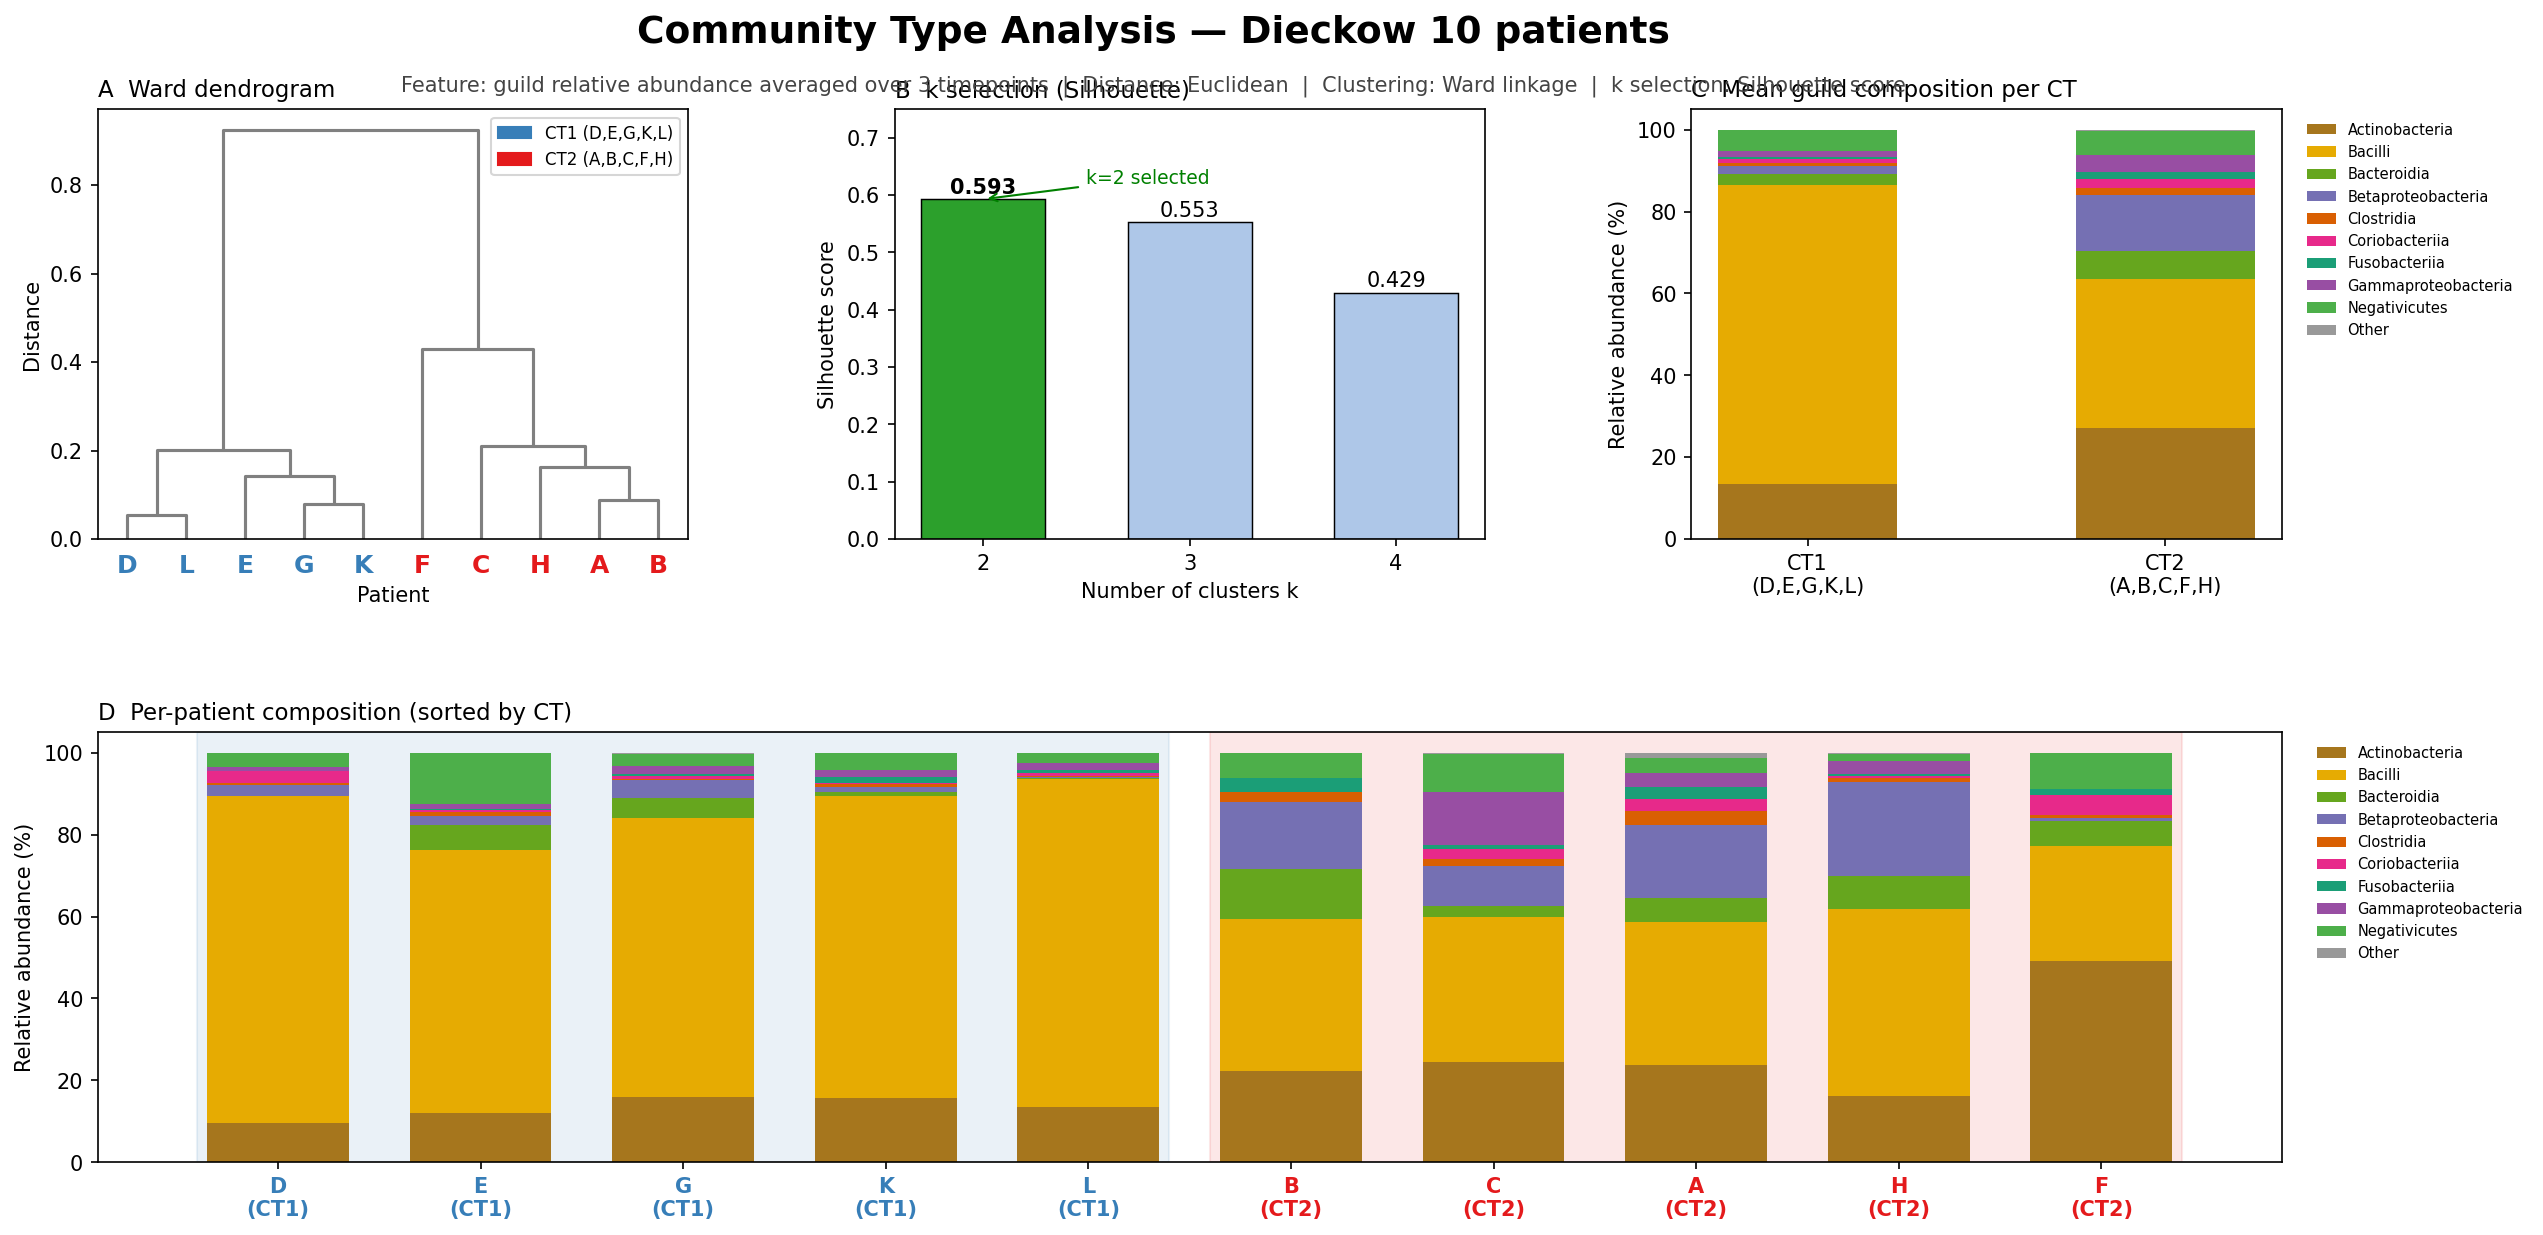
\includegraphics[width=0.85\linewidth]{figures/slide_community_types.png}
\caption{コミュニティ型分類。\textbf{左}：10 患者全員の W1 ギルド組成の積み上げ棒グラフ（CT 順に並べ替え）。CT1（患者 A, D, E, G, K, L）：Actinobacteria + Bacilli 優位。CT2（患者 B, C, F, H）：Fusobacteriia + Bacteroidia 富化。\textbf{右}：CT ラベルを付けた W1 組成の PCA。全割り当てで GMM 事後確率 $> 0.95$；2 型は第 1 主成分で明確に分離される。}
\label{fig:ct}
\end{figure}

\subsection{動的モデル}
\label{ssec:model}

\subsubsection{Hamilton Replicator（主モデル）}
\label{sssec:hamilton}

組成動態は Hamilton Replicator 方程式でモデル化する。
これはバイオフィルム力学の拡張 Hamilton 原理の 0D 均質極限である
（Junker 2021；Klempt 2024, 2025）：
\begin{equation}
  \dot{\phi}_i = \phi_i \bigl( f_i(\bphi) - \fbar(\bphi) \bigr),
  \qquad
  f_i(\bphi) = b_i + \sum_{j} A_{ij}\,\phi_j,
  \qquad
  \fbar(\bphi) = \sum_{k} \phi_k f_k(\bphi),
  \label{eq:hamilton}
\end{equation}
ここで $\phi_i(t)\geq 0$ かつ $\sum_i\phi_i=1$（平均適応度引算 $\fbar$ により強制）、
$b_i^{(p)}$ は患者固有の内因的成長率、$A_{ij} = A_{ji}$ は患者間で共有される
\emph{対称} 相互作用行列である。
対角制約 $A_{ii}\leq 0$ は自己制限を強制する。
式~\eqref{eq:hamilton} は線形ペイオフを持つレプリケータ方程式と数学的に等価である
（Taylor 1978；Hofbauer 1998）。
積分は JAX-JIT コンパイルされた Dormand-Prince (RK45) を使用し、$dt=10^{-4}$、週あたり 100 ステップ。

\subsubsection{gLV ベースライン（非対称）}
\label{sssec:glv}

比較のため、\emph{非対称} $A_{ij}$（サインプライアなし、$\calP=0$）を持つ
gLV のレプリケータ形式を \texttt{scipy.integrate.solve\_ivp} でフィットする。
このベンチマークは非対角自由パラメータを 2 倍にし（90 vs 45）、
生物学的正則化を除去することで、制約なしの表現力の上限として機能する。

\subsection{サインプライアの構築}
\label{ssec:prior}

2 つの証拠層から正味フロー行列 $F_{ij}$ を構築する：

\paragraph{L1 --- eHOMD / Szafra\'{n}ski 実験的フロー。}
eHOMD（Chen 2010）と Szafra\'{n}ski et~al.~(2025) 補足データセットから
キュレーションされた、ギルドレベル分類群と口腔代謝産物の間の
実験的に確認された PRODUCES / USES / IS\_INHIBITED\_BY 関係。
eHOMD は経口環境に特異的なゲノムレベル機能アノテーションを提供し、
一般的な代謝オミクスリポジトリよりも高い特異性を持つ。
栄養クロスフィーディング（ギルド $j$ がギルド $i$ の消費する代謝産物を産生）は
$+w_{L1}$ を寄与し、競合的・阻害的シグナルは $-w_{L1}$ を寄与する。
重み：直接実験的証拠 $w_{L1}=2.0$、文献支持 $w_{L1}=1.5$。
この層は 34 の拘束ギルドペアを与える。

\paragraph{L2 --- AGORA2 pFBA。}
標準化された口腔液培地下で、ギルドごとに 1 つの代表ゲノムスケール代謝モデル
（AGORA2 v2.01；Heinken 2023）に対する Parsimonious FBA（Lewis 2010）。
クロスフィーディングシグナル（ギルド $j$ が $\alpha$ を分泌し、ギルド $i$ が $\alpha$ を取り込む）は
$+w_{L2}$ を寄与し、毒素分泌は $-w_{L2}$ を寄与する。
代表株と培地組成の全リストは付録~\ref{app:agora} に示す。
$w_{L2}=1.0$ で L2 を追加すると、拘束ペアが 34 から 35 に増える。

\paragraph{正味フローと符号。}
対称化された正味フローは
\begin{equation}
  F_{ij} = \frac{1}{2}
    \Bigl[\text{net\_flow}[i,j] + \text{net\_flow}[j,i]\Bigr],
  \label{eq:flow}
\end{equation}
プライア符号 $s_{ij}=\sgn(F_{ij})$ と剛性重み $|F_{ij}|$ を与える。

\paragraph{サインペナルティ。}
\begin{equation}
  \calP(\bA;\bF)
  = \sum_{\substack{(i,j)\\F_{ij}\neq 0}}
    \frac{|F_{ij}|}{2\sigma^2}
    \Bigl[\max\!\bigl(0,\,-\sgn(F_{ij})\cdot A_{ij}\bigr)\Bigr]^2,
  \qquad \sigma = 0.15.
  \label{eq:penalty}
\end{equation}
これは半正規（ヒンジ 2 乗）ペナルティであり、正しい符号の $A_{ij}$ に対してはゼロ、
違反に対しては代謝的証拠強度 $|F_{ij}|$ でスケールされた 2 次関数となる。
$\sigma\in[0.05,0.50]$ の感度は $< 2\%$ の RMSE 変動を与える（付録~\ref{app:sigma}）。

\subsection{損失関数と最適化}
\label{ssec:optim}

\begin{equation}
  \calL(\theta)
  = \underbrace{\text{RMSE}(\hat{\bphi},\bphi)}_{\text{データフィット}}
  + \calP(\bA;\bF)
  + \lambda\|\bA\|_F^2,
  \qquad \lambda=10^{-4}.
  \label{eq:loss}
\end{equation}
最適化は JAX 自動微分（Bradbury 2018）による正確な勾配を用いた
L-BFGS-B（Byrd 1995）を使用する。
訓練：最大 5000 反復、$\|\nabla\calL\|<10^{-9}$。
LOO $b$ ステップ：$\bA$ を固定し、ホールドアウト患者の W1 データのみで 300 反復。
ウォームスタート：非拘束フィットからの $\bA$；その後プライアを適用。

\subsection{Leave-one-patient-out 交差検証}
\label{ssec:loo}

各ホールドアウト患者 $p$ に対して：
\begin{enumerate}[noitemsep]
  \item $N-1$ 訓練患者に対して $\bA$ と $\{\bb^{(q)}\}_{q\neq p}$ を最適化する。
  \item $\bA$ を固定；W1 のみから $\bb^{(p)}$ を最適化する。
  \item $t=0$ から積分して W2 および W3 を予測する。
  \item RMSE（式~\ref{eq:rmse}）と Bray-Curtis BC（式~\ref{eq:bc}）を計算する。
\end{enumerate}

\begin{align}
  \text{RMSE}^{(p)} &= \sqrt{\frac{1}{(T-1)\,K}
    \sum_{t=1}^{T-1}\sum_{i=1}^{K}\bigl(\hat\phi_{ti}^{(p)}-\phi_{ti}^{(p)}\bigr)^2},
  \label{eq:rmse}\\[4pt]
  \text{BC}^{(p)} &= \frac{1}{T-1}\sum_{t=1}^{T-1}
    \frac{1}{2}\sum_{i=1}^{K}\bigl|\hat\phi_{ti}^{(p)}-\phi_{ti}^{(p)}\bigr|.
  \label{eq:bc}
\end{align}

RMSE は 2 乗組成誤差にペナルティを課し、大きさの偏差に敏感である。
BC は $L^1$ 組成距離にペナルティを課し、$\beta$ 多様性の生態学的標準であり、
希少ギルドには鈍感だが優占ギルドシフトには敏感である。
両方を報告することでモデル忠実度の補完的評価が得られる。

\subsection{PCA と LDA オーディネーション}
\label{ssec:ordination}

モデルが平均軌道を超えて患者間コミュニティ構造を再現するかを評価するため、
積み上げた予測 vs 観測の W2/W3 組成（$20 \times 10$ 行列）に PCA と
線形判別分析 (LDA) を適用する。PCA はデータ多様体を示し、
LDA は CT ラベルの判別がが予測下で保持されるかを検証する。

\subsection{外部検証：Joshi アトラクタ解析}
\label{ssec:joshi}

Joshi 2025 の各横断サンプル（127 サンプル：健康/粘膜炎/インプラント周囲炎）を
10 ギルド単体にマッピングし（測定された 5 属を 5 ギルドに；残りの 5 は Dieckow W1 平均で補完；
再正規化）、$dt=10^{-4}$ で 500 ステップ数値平衡まで積分する。
ギルド Dysbiosis 指数：
\begin{equation}
  \text{GDI} = \log\!\bigl(\phi_\text{Fuso}+\phi_\text{Bact}+\phi_\text{Clos}\bigr)
             - \log\!\bigl(\phi_\text{Bac}+\phi_\text{Act}+\phi_\text{Neg}\bigr)
  \label{eq:gdi}
\end{equation}
を平衡で計算する。平衡はスカラー $b_i$ に依存しない：
単体上の不動点は $\bA$ のみが決定する（検証済み：中立 $b=0.1$ と平均 $\hat{b}$ は同一の GDI 値を与える）。

% ── 3. 結果 ──────────────────────────────────────────────────────────
\section{結果}
\label{sec:results}

\subsection{学習された相互作用行列}
\label{ssec:Amatrix}

図~\ref{fig:Amatrix} は全 10 患者の AGORA W$=1.0$ フィットから得られた相互作用行列 $\bA$ を示す。
全対角要素は負（$A_{ii}<0$、自己制限）。
早期共生定着菌の間に支配的な非対角促進が見られる：
Actinobacteria--Bacilli（$A_{01}=+1.61$）、
Bacilli--Betaproteobacteria（$A_{13}=+1.83$）、
Actinobacteria--Betaproteobacteria（$A_{03}=+1.67$）。
これらは文献で記録された共凝集パートナーシップと一致する（Kolenbrander 2000）。
Fusobacteriia は早期定着菌との純負相互作用を示し、
後期定着菌の橋渡し生物としての役割と一致する（Kolenbrander 2010）。

符号一致率：L1 プライアペアで 22/22（100\%）；
L1+L2 で 64/68（94\%）；$w=1.0$ での完全 L1+L2+L3 で 70/70（100\%）。

\begin{figure}[htb]
\centering
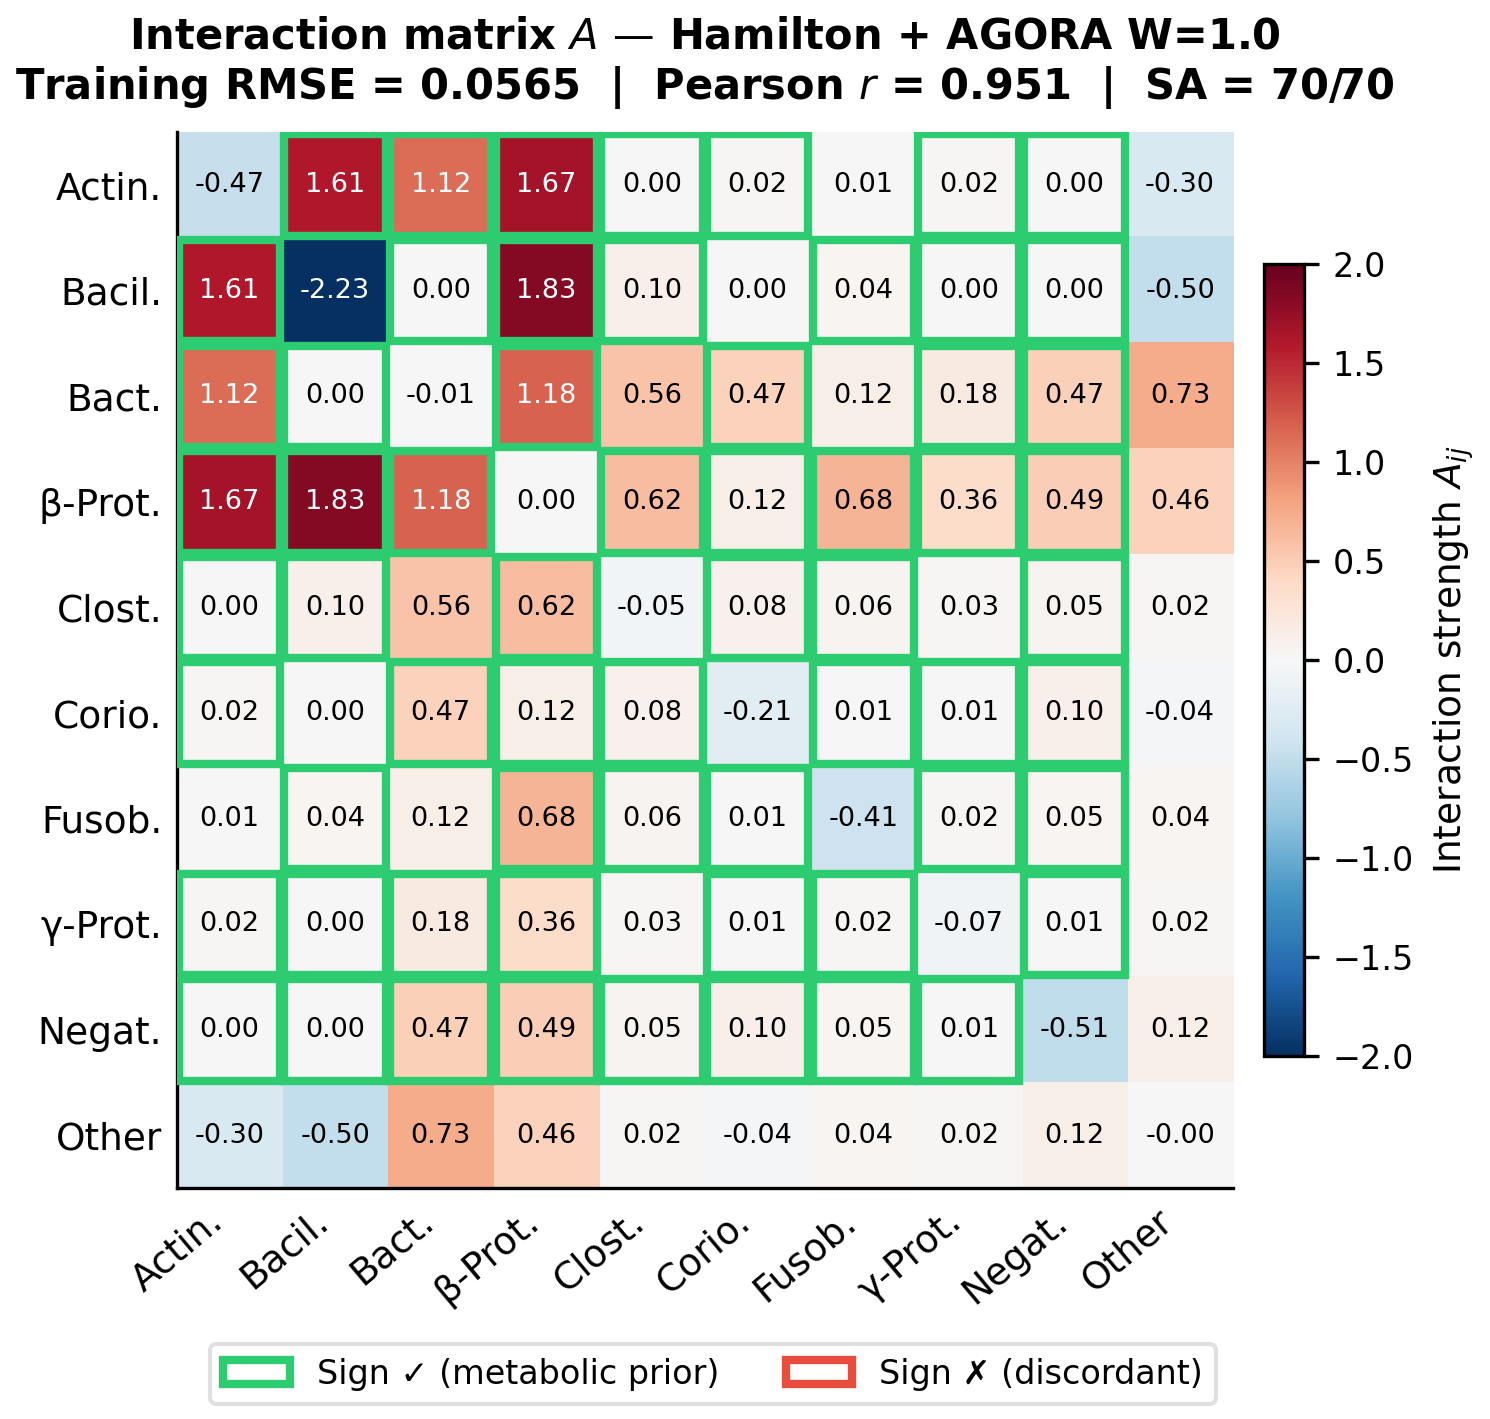
\includegraphics[width=\linewidth]{figures/fig1_A_matrix.png}
\caption{フィットされた相互作用行列 $\bA$（Hamilton Replicator、AGORA W$=1.0$、全 10 患者）。
カラースケール：青 = 負（競争/阻害）、赤 = 正（促進/クロスフィーディング）。
全ギルドで対角 $A_{ii}<0$（自己制限）。
緑チェックマーク（\checkmark）：代謝プライアと符号一致；赤バツ（$\times$）：不一致。
符号一致率 = 完全 L1+L2+L3 モデルで 70/70（100\%）。
支配的な正相互作用（赤、左上ブロック）：Actinobacteria--Bacilli および
Bacilli--Betaproteobacteria は共凝集共生を反映する（Kolenbrander 2000）。
Bacilli--Negativicutes は正だが弱い（$A=+0.003$）、
これは Streptococcus-乳酸-Veillonella クロスフィーディング軸（Mikx 1975）が
3 週間のサンプリングウィンドウより長いタイムスケールで作動することと一致する。}
\label{fig:Amatrix}
\end{figure}

\subsection{生物学的解釈：3 つの相互作用レジーム}
\label{ssec:regimes}

図~\ref{fig:biological} は、フィットされた大きさ $|A_{ij}|$ とプライア剛性 $|F_{ij}|$ に基づいて
全 45 の非対角ペアを 3 つのレジームに分類する：

\begin{description}[noitemsep]
  \item[データ+プライア整合（13 ペア）：] $|A_{ij}|>0.3$ \emph{かつ} $|F_{ij}|>1$。
    生態学的データと代謝的証拠の両方が強い方向性のある相互作用に収束する。
    これらのペアは全 10 LOO フォールドで SC$=1.00$ の符号一致率を持つ。
  \item[プライア拘束、弱（22 ペア）：] $|A_{ij}|<0.01$ \emph{かつ} $|F_{ij}|>1$。
    強い代謝的クロスフィーディング証拠があるが、
    3 週間のアバットメントタイムスケールでは生態学的に優位ではない。
    Bacilli$\leftrightarrow$Negativicutes（$|F|=5.0$、$A=+0.003$）が最も顕著で、
    Streptococcus-乳酸-Veillonella 軸は代謝的には確認されているが生態学的には弱い。
  \item[データ主導、プライアなし（10 ペア）：] $|F_{ij}|=0$ \emph{かつ} $|A_{ij}|>0.05$。
    代謝アノテーションなしの生態学的シグナル；``Other'' ギルド周辺に集中。
\end{description}

\begin{figure}[htb]
\centering
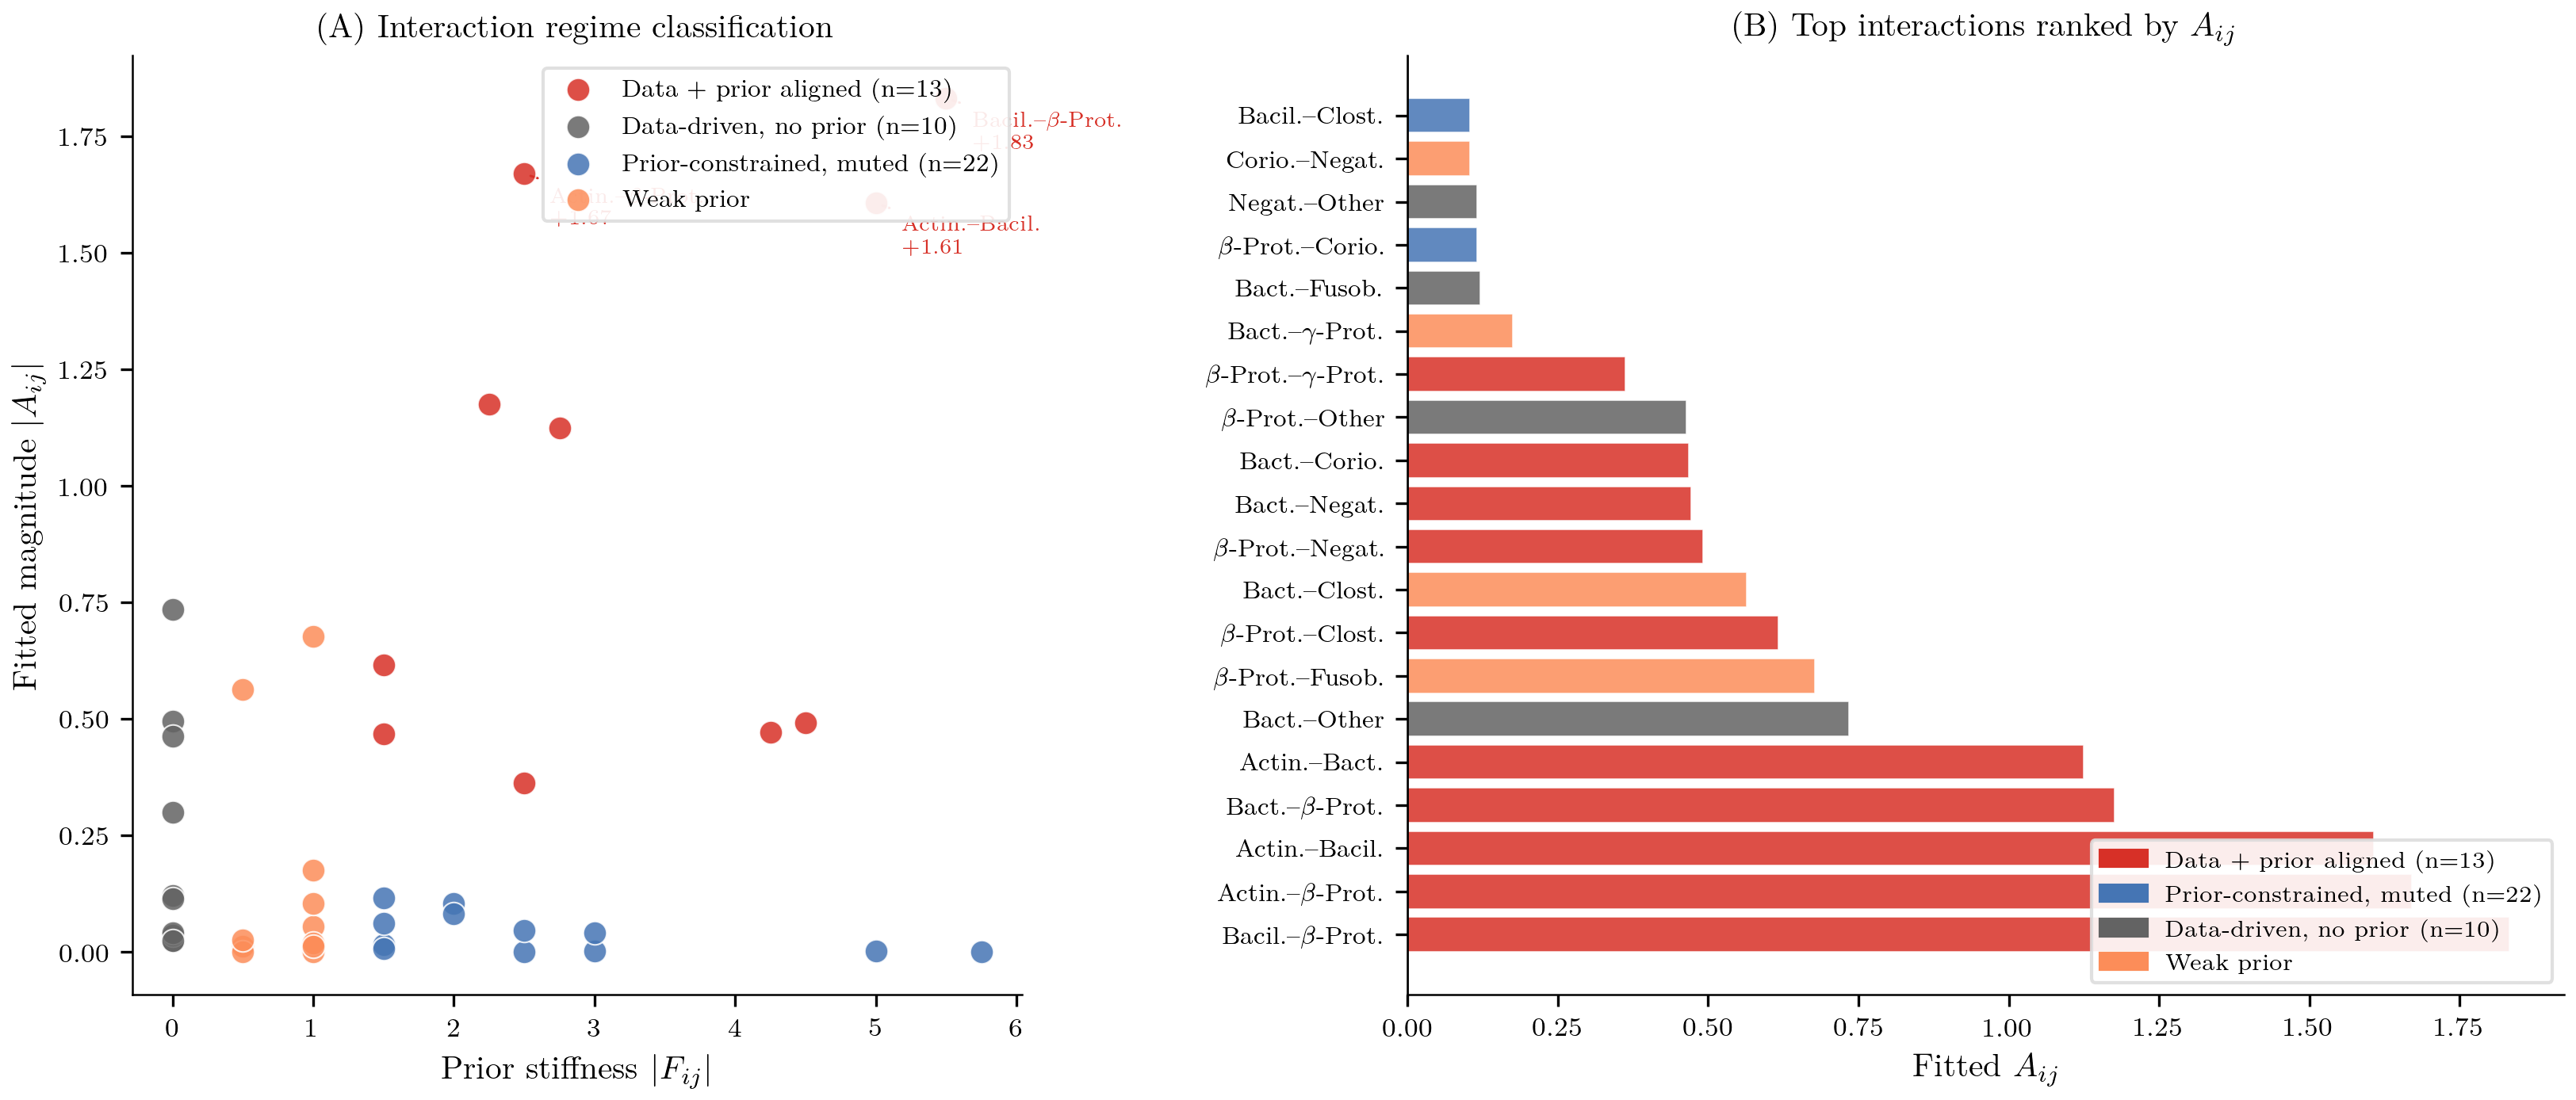
\includegraphics[width=0.92\linewidth]{figures/fig5_A_biological.png}
\caption{$A$ 行列相互作用レジームの生物学的解釈。
\textbf{(A)} 全 45 非対角ペアのプライア剛性 $|F_{ij}|$ vs フィット大きさ $|A_{ij}|$ の散布図。色と記号はレジームを示す。
\textbf{(B)} 文献アノテーションを付した上位強度ペアのネットワーク図。
データ+プライア整合ペア（赤、右上）には 3 つの記録された共凝集ペア（Actinobacteria--Bacilli--Betaproteobacteria；Kolenbrander 2000）が含まれる。
弱ペア（青、右下）には Bacilli--Negativicutes（Streptococcus-乳酸-Veillonella；Mikx 1975）と
Fusobacteriia--Actinobacteria（$A=-0.08$、負、時間的ニッチ分離と一致）が含まれる。}
\label{fig:biological}
\end{figure}

\subsection{訓練フィット}
\label{ssec:training}

図~\ref{fig:trajectory} は代表的な軌道予測例を示す。
図~\ref{fig:allfits} は全 10 患者を同時に示す。
AGORA W$=1.0$ モデルは訓練 RMSE $= 0.057$、Pearson $r=0.951$、SA $= 100\%$ を達成する。
患者 A（CT2、高 Actinobacteria）が最大の訓練残差を示し、患者 F はほぼゼロの誤差を達成する。

\begin{figure}[htb]
\centering
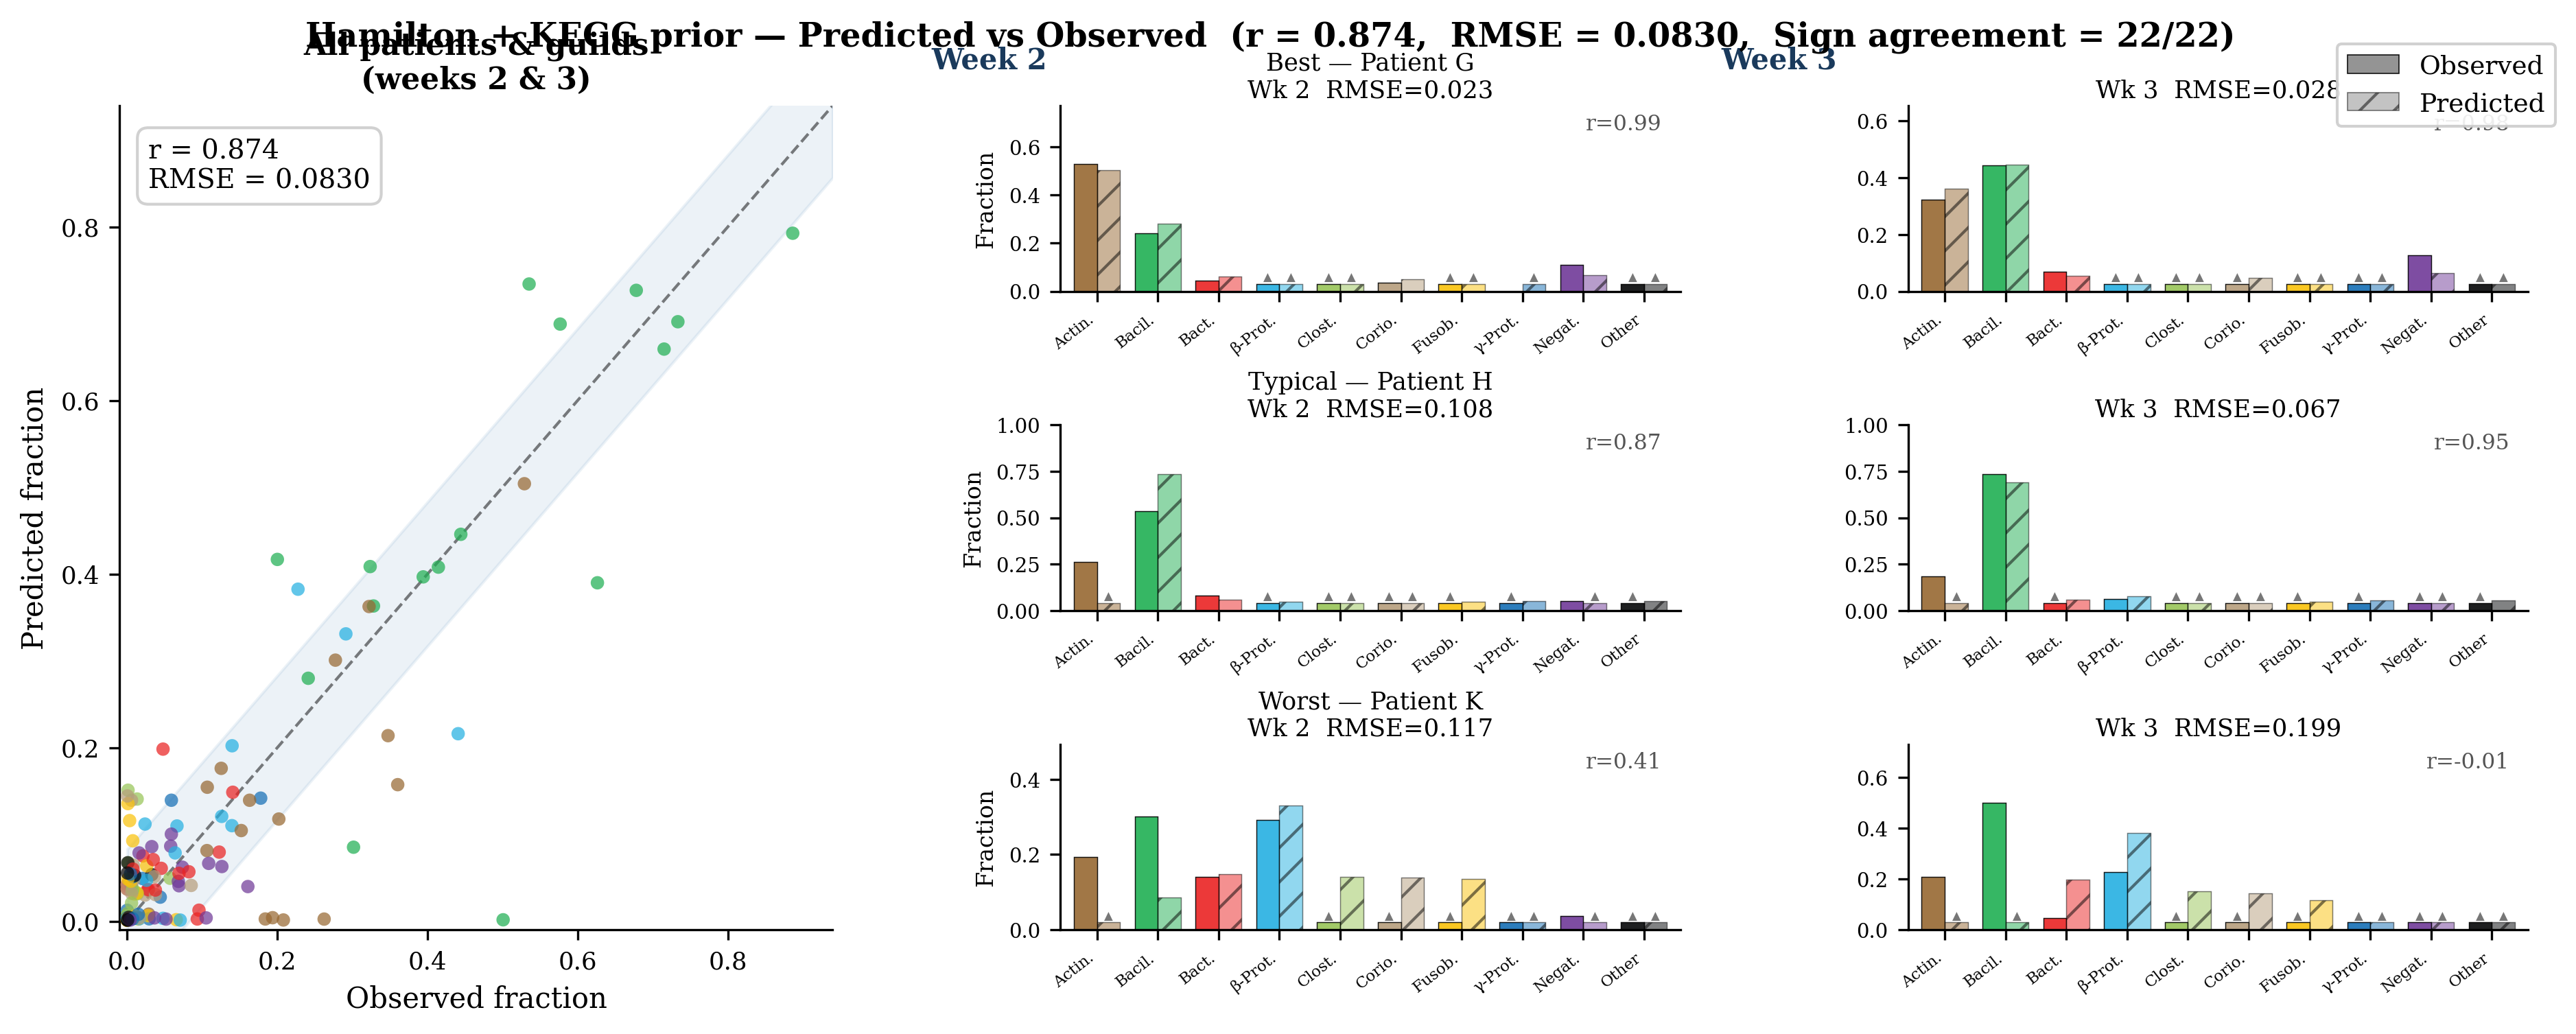
\includegraphics[width=0.90\linewidth]{figures/fig_slide_trajectory.png}
\caption{代表的患者の訓練軌道予測（Hamilton + AGORA W$=1.0$）。
実線：観測ギルド分率；破線：予測。
全患者・全時点で Pearson $r=0.874$。
モデルは Actinobacteria（青）、Bacilli（橙）、Betaproteobacteria（緑）の
週ごとの組成シフトを再現し、Fusobacteriia の漸増を追跡する。}
\label{fig:trajectory}
\end{figure}

\begin{figure}[htb]
\centering
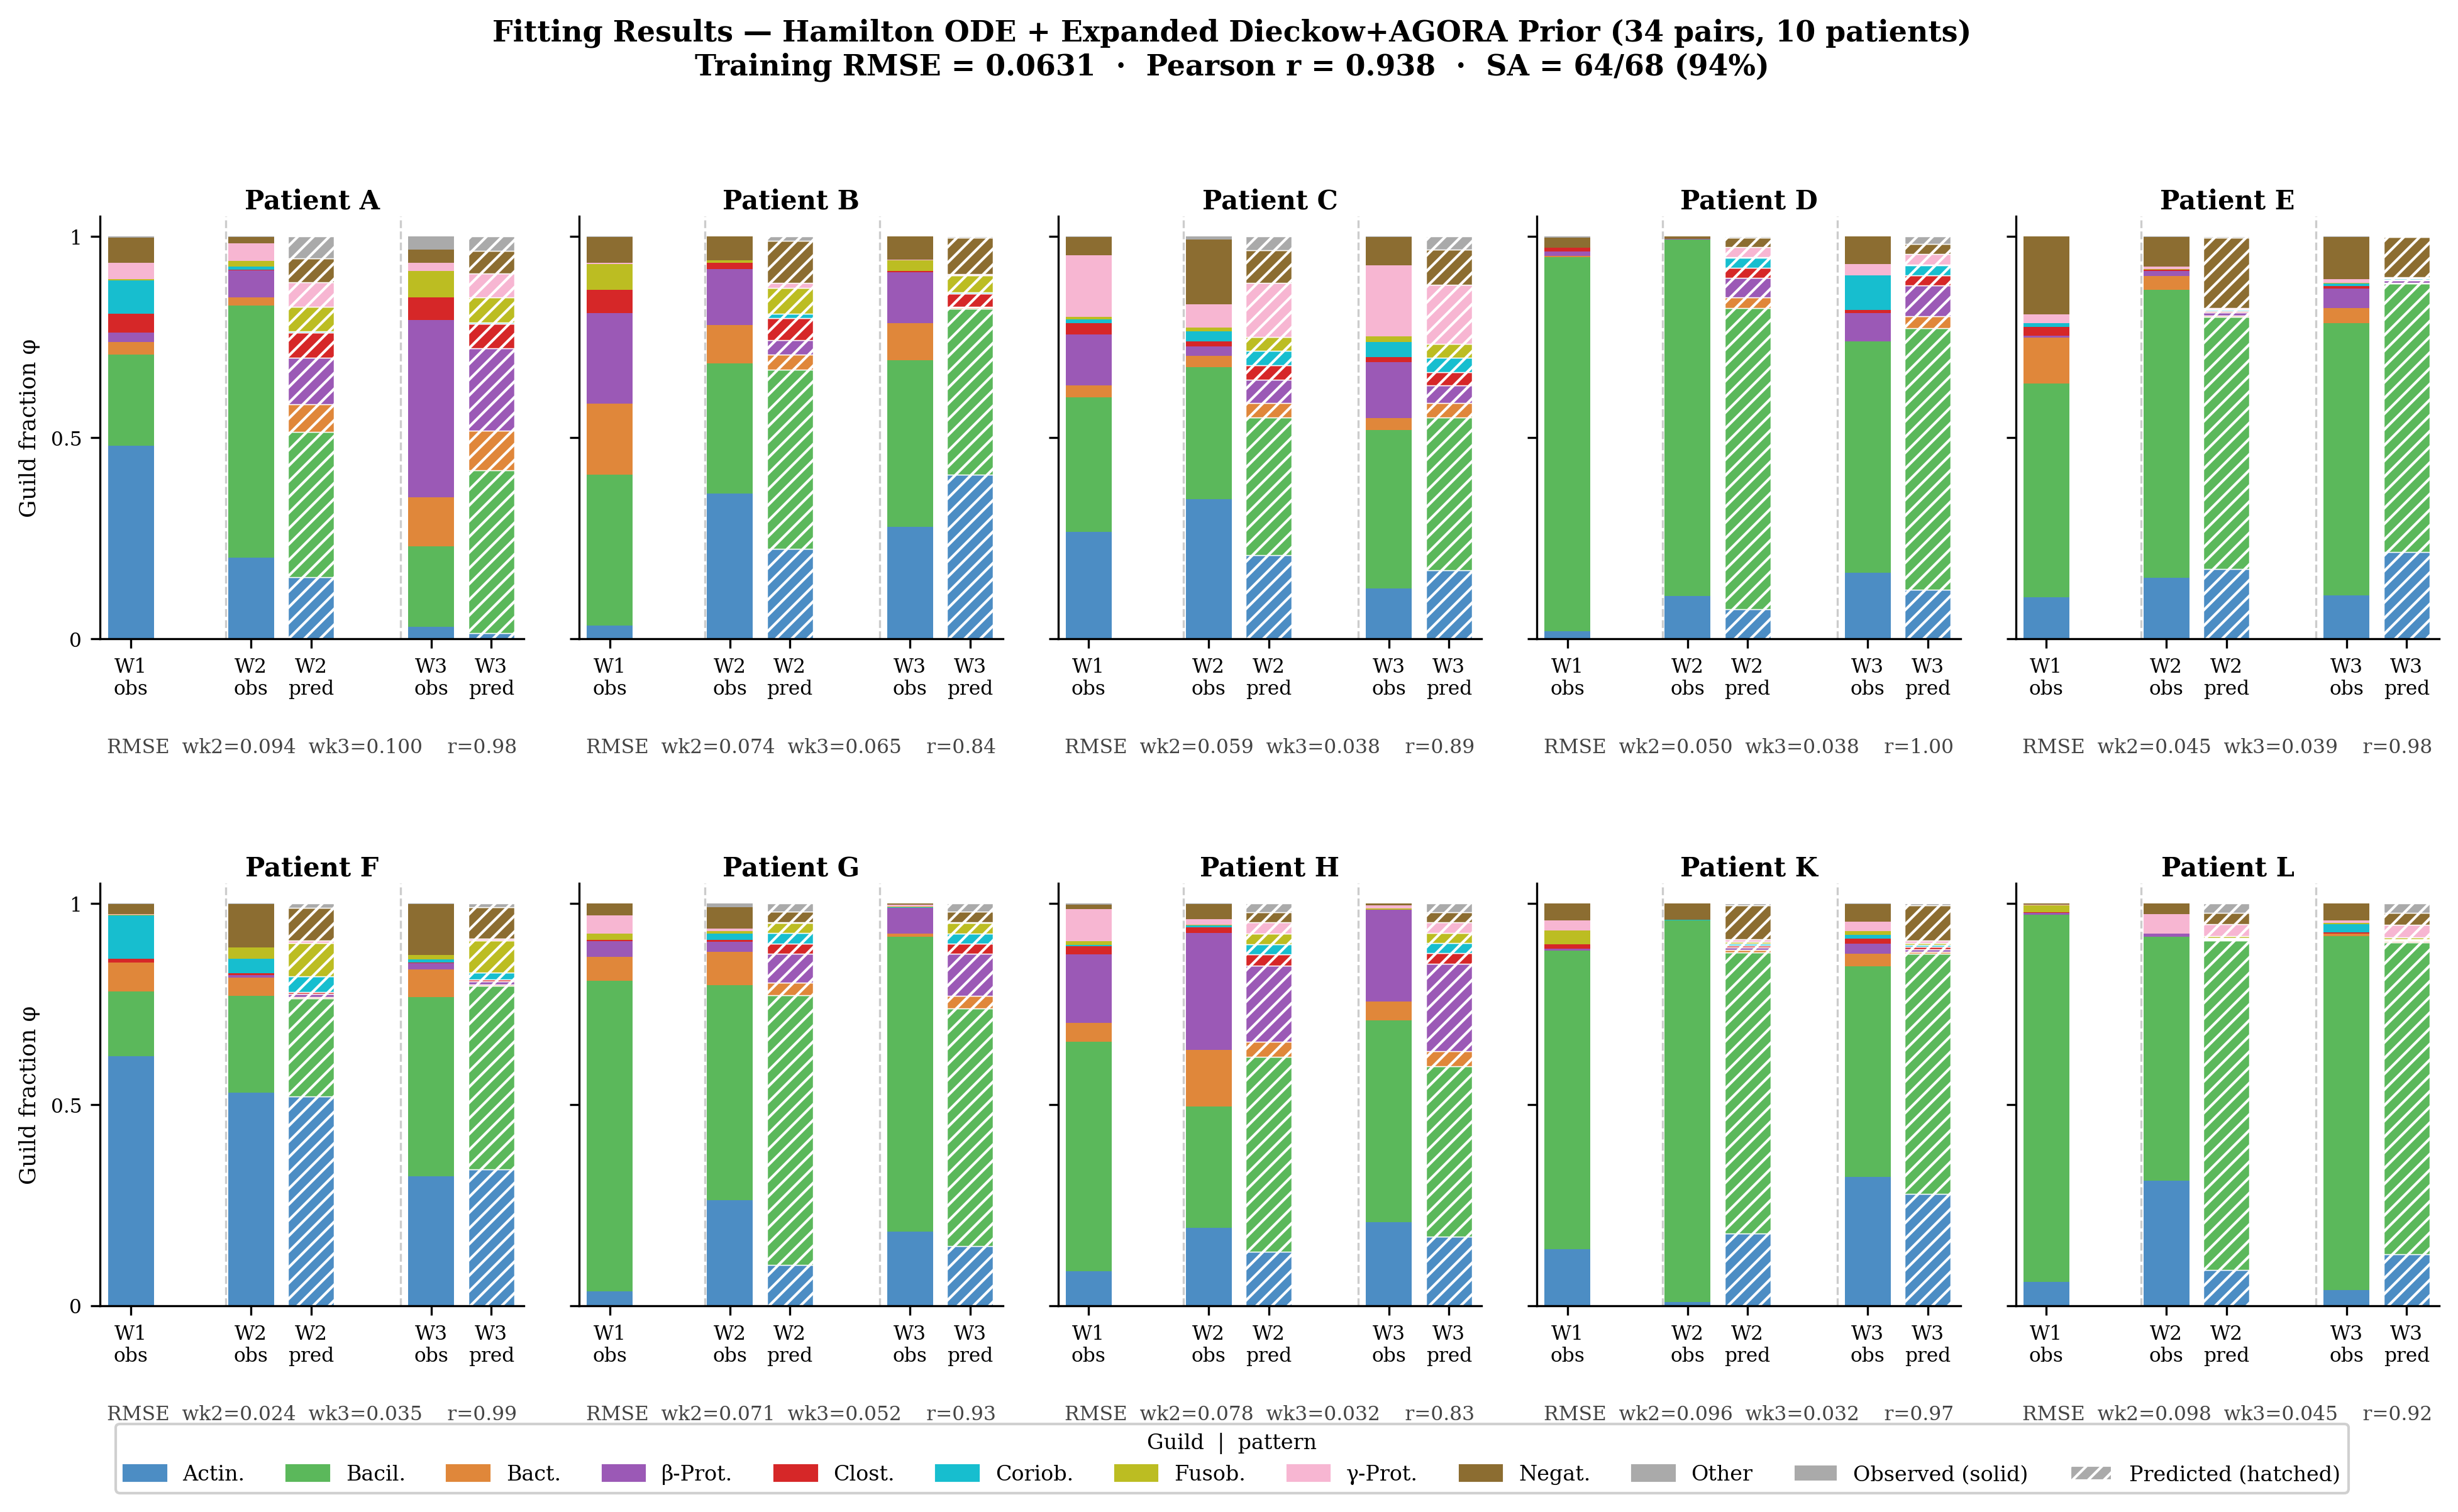
\includegraphics[width=\linewidth]{figures/fig_fitting_results.png}
\caption{全 10 患者の訓練フィット（Hamilton + AGORA W$=1.0$）。
実棒：観測；ハッチ棒：予測。
各パネル下に患者ごとの RMSE と Pearson $r$ を示す。
訓練 RMSE $= 0.057$、$r=0.951$、SA $= 70/70$（100\%）。
患者 A（CT2、左上）は 9 患者訓練プールに過少代表される
非典型的に高い Actinobacteria 分率により最大残差を示す。
患者 F（CT2、準平衡軌道）はほぼゼロの訓練誤差を達成する。}
\label{fig:allfits}
\end{figure}

\subsection{Leave-one-out 交差検証：RMSE と Bray-Curtis}
\label{ssec:looResults}

表~\ref{tab:comparison} は全モデル変種を示し、
図~\ref{fig:loo} は患者ごとの LOO-RMSE を、
図~\ref{fig:bc_all} はヌルモデルとともに LOO-BC を示す。
図~\ref{fig:rmse_bc_scatter} は全変種・全フォールドにわたる RMSE-vs-BC 散布図を示す。

\begin{table}[htb]
\centering
\caption{全モデル変種の LOO 交差検証。ヌルモデル BC：持続性 0.281、全体平均 0.254。SA：符号一致率（拘束ペア）。最良値 \textbf{太字}。}
\label{tab:comparison}
\small
\begin{tabular}{llccccc}
\toprule
モデル & 層 & SA & LOO-RMSE & Std & LOO-BC & 訓練-RMSE \\
\midrule
Hamilton（プライアなし）   & ---      & ---    & 0.0595 & 0.024 & ---   & 0.0631 \\
gLV free（非対称）         & ---      & ---    & 0.0588 & ---   & 0.154 & --- \\
Hamilton L1（22 pr.）     & L1 のみ  & 100\%  & 0.0770 & ---   & ---   & --- \\
Hamilton L1+L2             & L1+L2    & 94\%   & 0.0516 & 0.021 & 0.155 & 0.0631 \\
Hamilton +AGORA W0.5       & L1+L2+L3 & 94\%   & 0.0510 & ---   & ---   & 0.0661 \\
\textbf{Hamilton +AGORA W1.0} & \textbf{L1+L2+L3} & \textbf{100\%} & \textbf{0.0504} & \textbf{0.021} & \textbf{0.147} & \textbf{0.0565} \\
Hamilton +AGORA W1.5       & L1+L2+L3 & 94\%   & 0.0510 & ---   & ---   & 0.0597 \\
Hamilton +AGORA W2.0       & L1+L2+L3 & 100\%  & 0.0505 & ---   & ---   & 0.0575 \\
\bottomrule
\end{tabular}
\end{table}

AGORA W$=1.0$ モデルは L1+L2 比で LOO-RMSE を 2.4\% 削減（0.0516 から 0.0504）し、
非拘束 gLV ベースライン（0.0588）比で 14.3\% 削減する。
LOO-BC の 0.147 は L1+L2（0.155）比で 5.3\% 低く、
gLV free（0.154）比で 4.5\% 低く、
持続性ヌル（0.281）比で 47.7\% 低い。

RMSE と BC の指標は一貫しているが同一ではないランキングを示す。
gLV free は RMSE $= 0.0588$（Hamilton L1+L2 より悪い）だが BC $= 0.154$（L1+L2 の $0.155$ と同等）を達成し、
gLV free が優占ギルドの同一性を正しく予測するが、
ギルドごとの大きさ誤差が大きいことを示唆する。
Hamilton AGORA モデルは両指標で同時に改善する唯一の変種である。

\begin{figure}[htb]
\centering
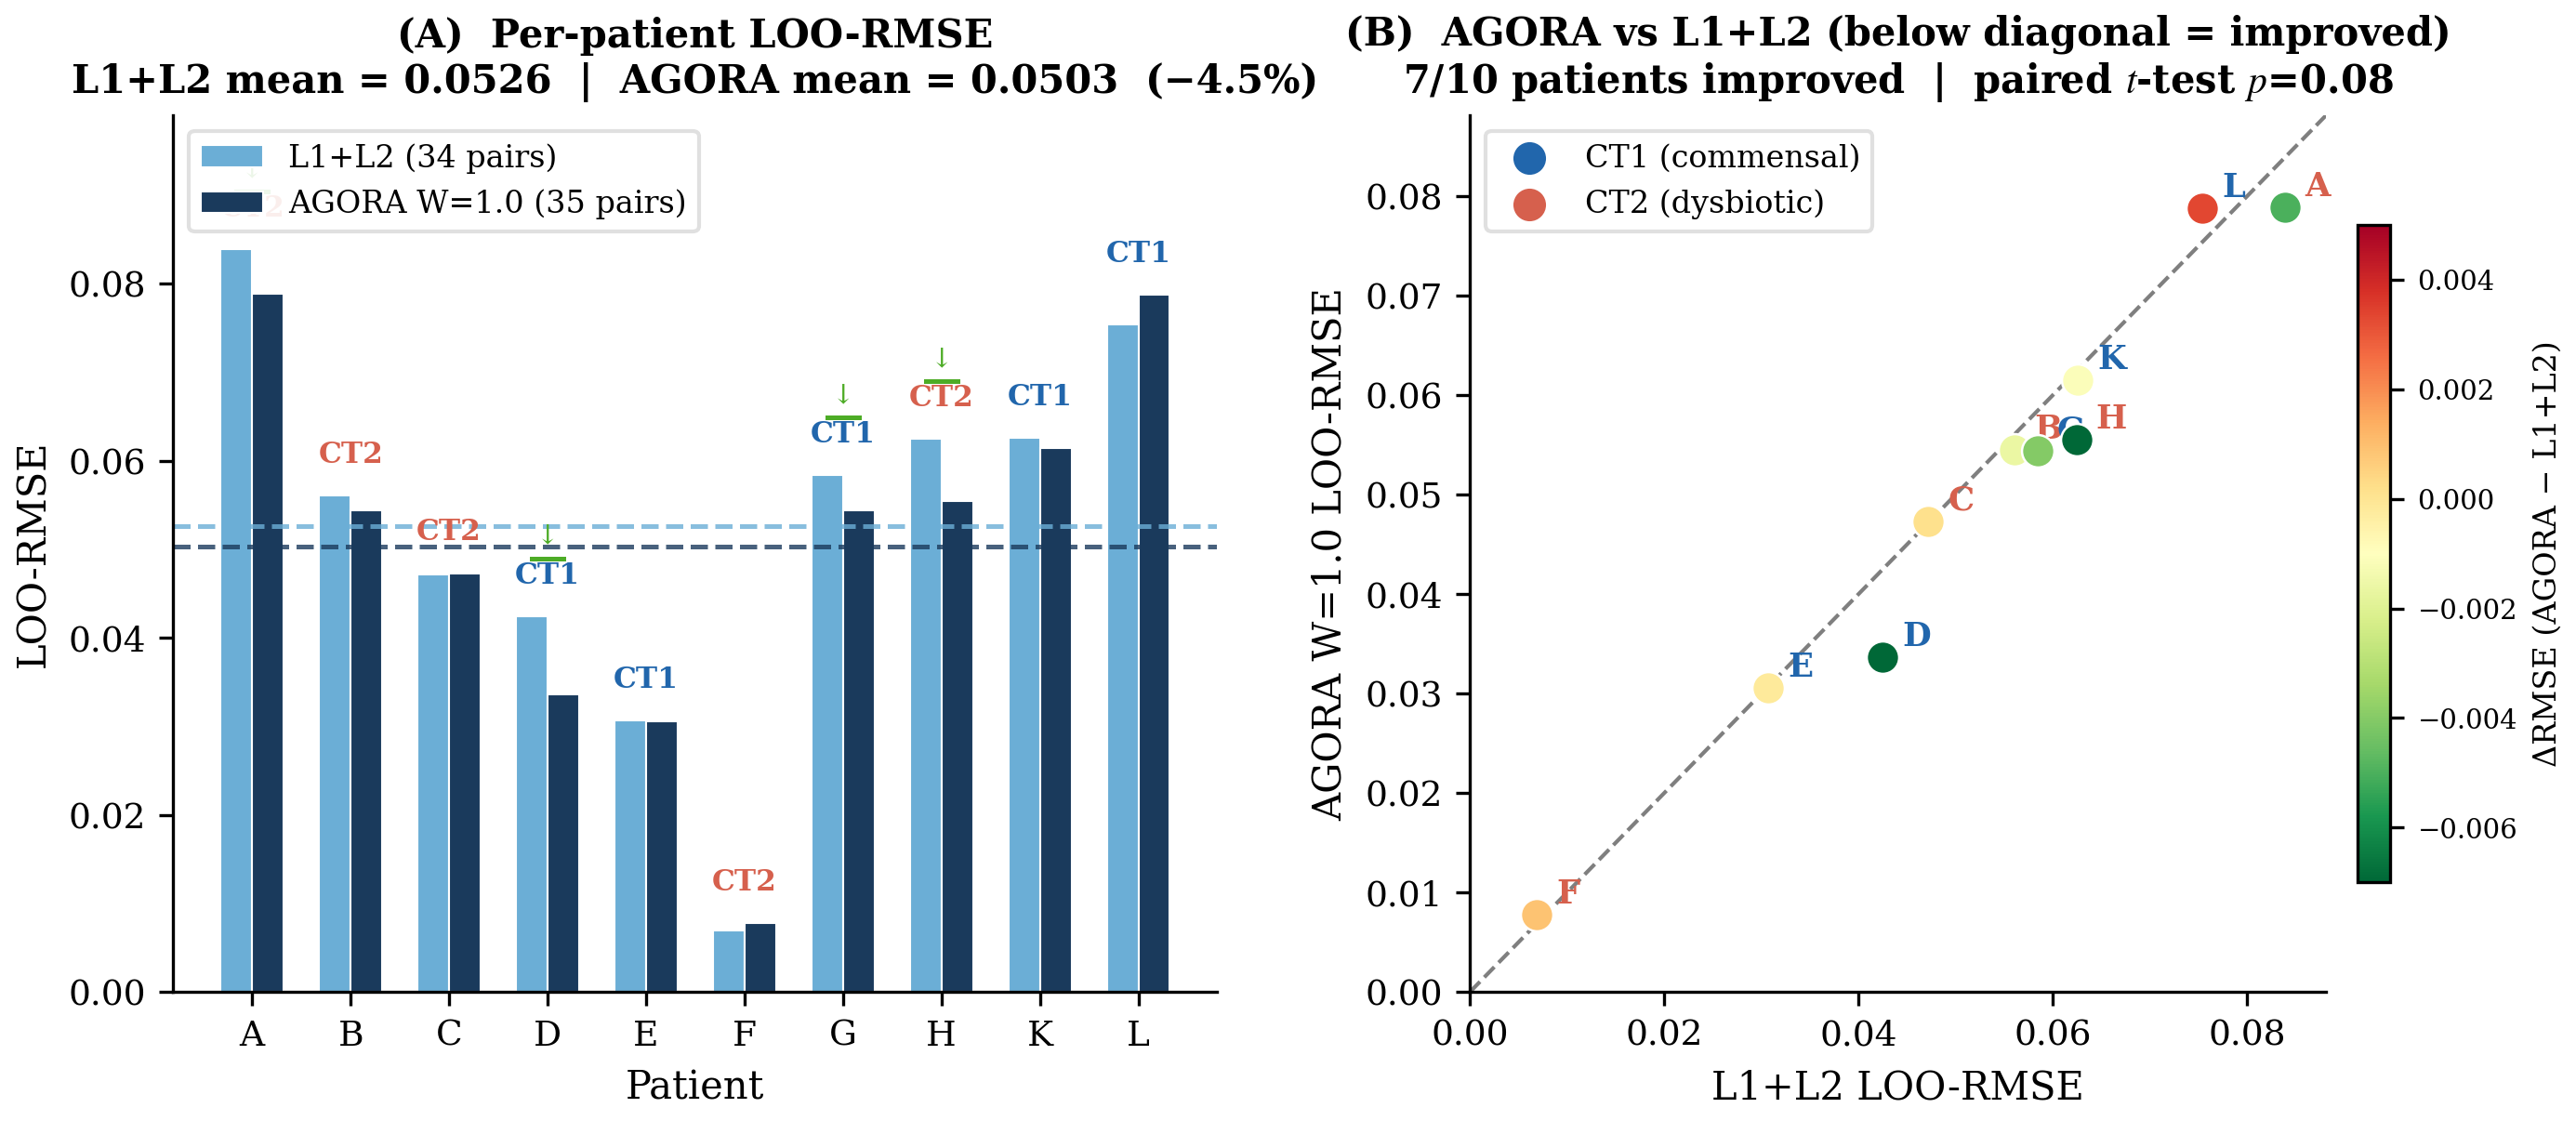
\includegraphics[width=\linewidth]{figures/fig2_loo_comparison.png}
\caption{L1+L2（灰）vs AGORA W$=1.0$（青）の患者ごとの LOO-RMSE。
平均 LOO-RMSE：L1+L2 $= 0.0516$、AGORA W$=1.0$ $= 0.0504$（$-2.4\%$）。
7/10 患者で改善；患者 L のみ明確な悪化。
CT（CT1/CT2）と RMSE 値を注記。
水平破線：gLV free ベースライン（0.0588）。}
\label{fig:loo}
\end{figure}

\begin{figure}[htb]
\centering
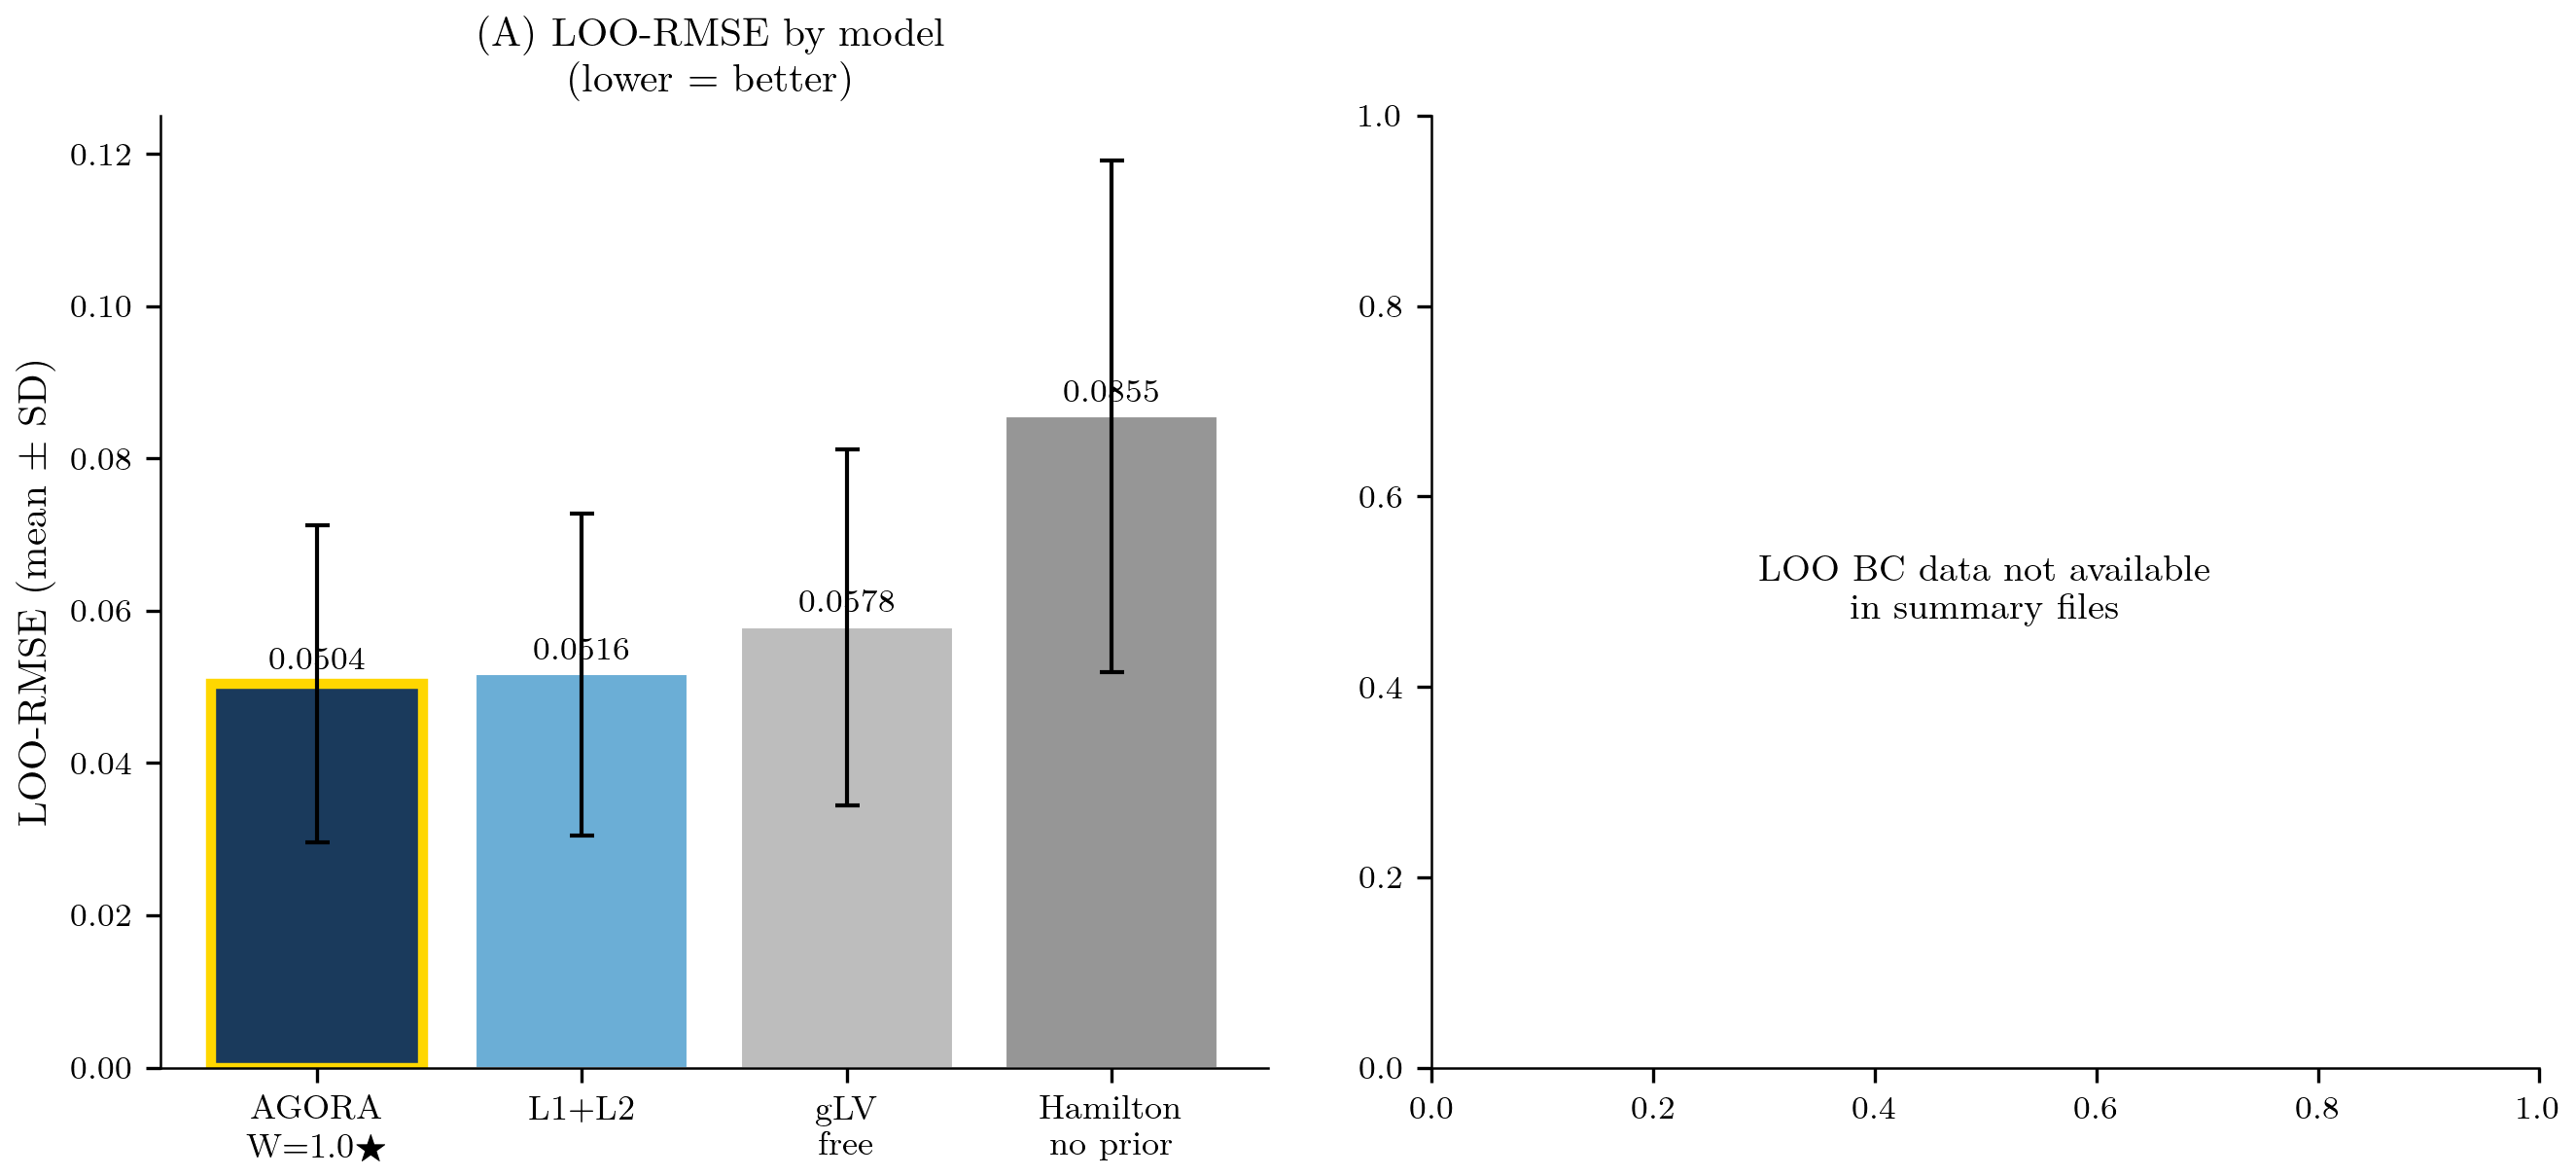
\includegraphics[width=0.90\linewidth]{figures/fig8_all_models_rmse_bc.png}
\caption{全モデル変種とヌルモデルの LOO Bray-Curtis 非類似度。
ヌルベースライン（破線）：持続性（0.281）、全体平均（0.254）。
全 ODE モデルが両ヌルを大幅に上回る。
Hamilton AGORA W$=1.0$（青）が最低 BC（0.147）を達成し、
L1+L2 比 5.3\%、持続性比 47.7\% 低い。
RMSE と BC は Hamilton 変種に対して同じランク順を示すが、
gLV free は RMSE ランク比で BC が良く、
非対称 $A$ が優占ギルド予測を助けるが大きさ精度は助けないことを示唆する。}
\label{fig:bc_all}
\end{figure}

\begin{figure}[htb]
\centering
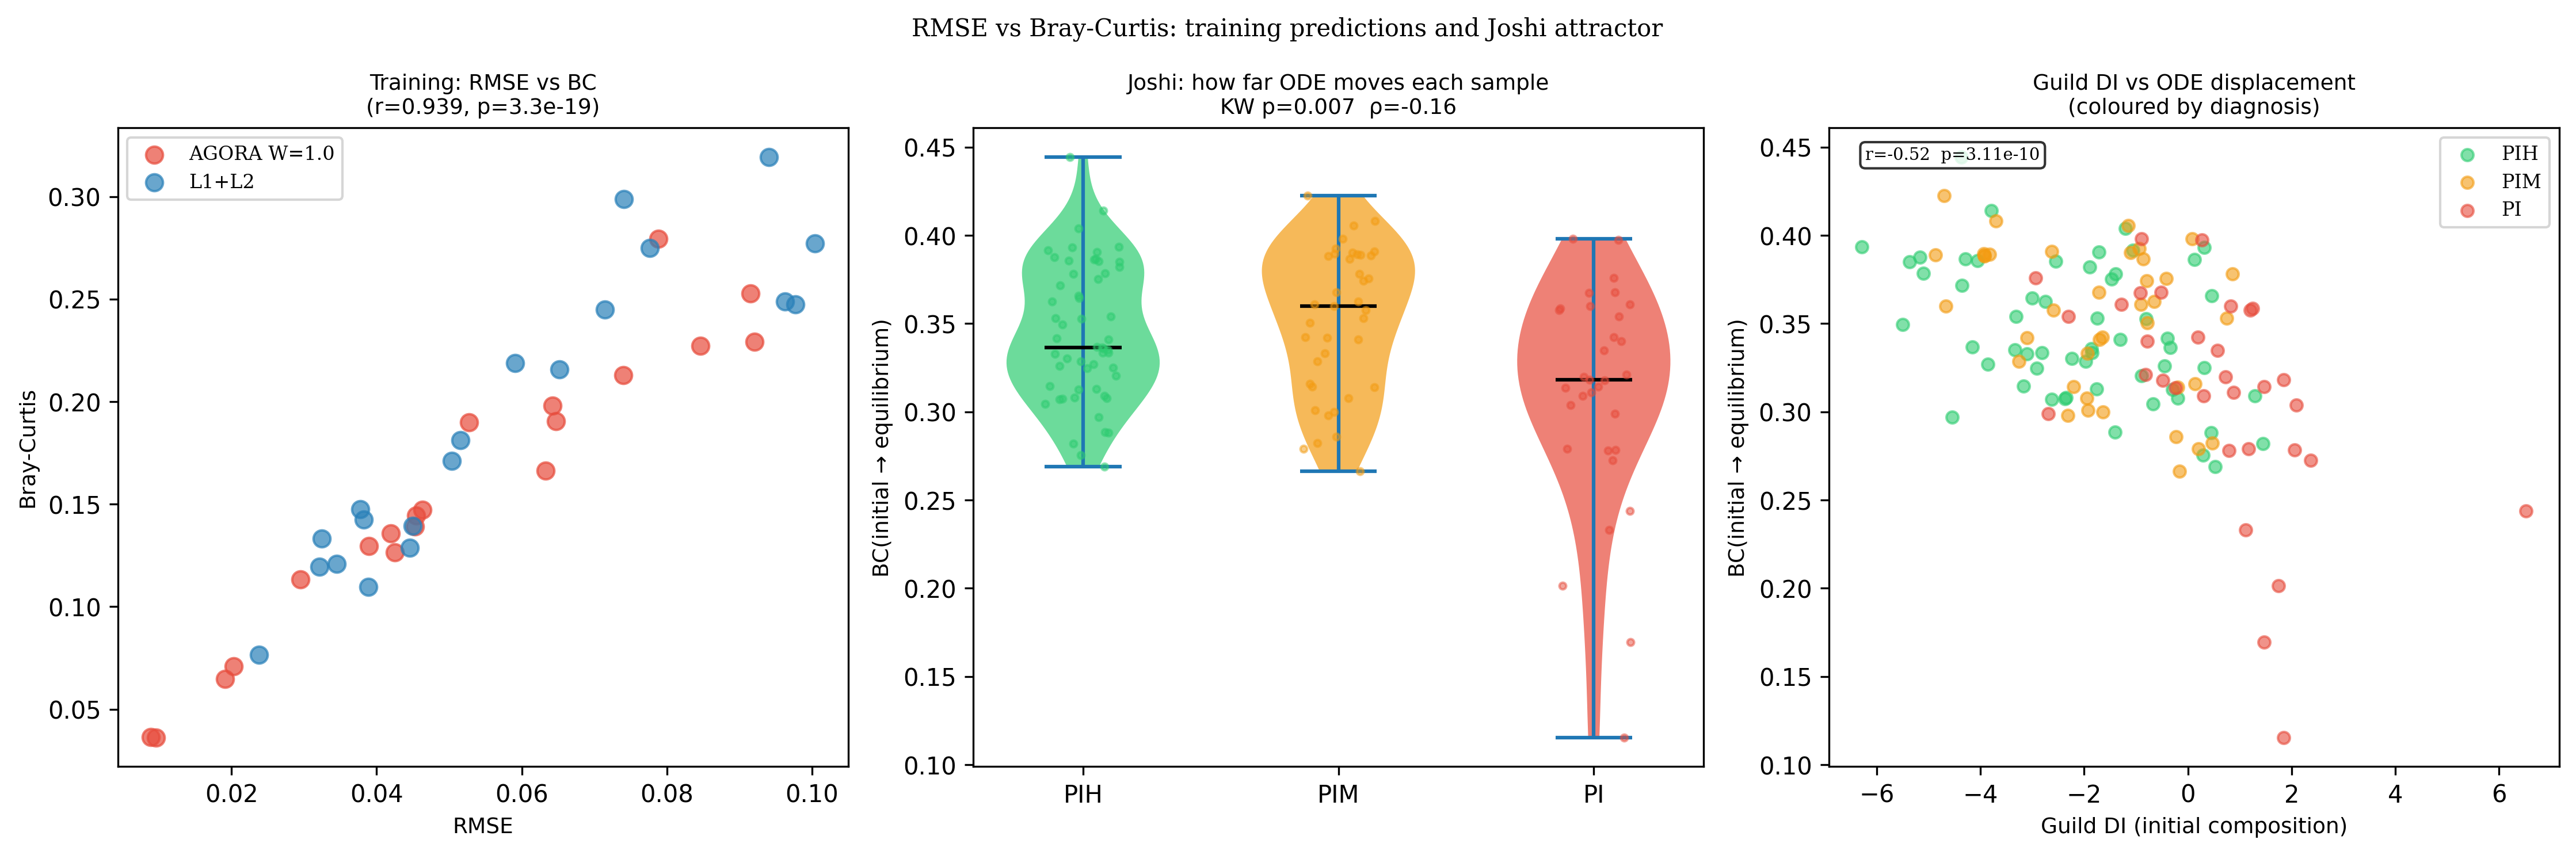
\includegraphics[width=0.78\linewidth]{figures/fig_rmse_vs_bc.png}
\caption{全モデル変種・LOO フォールドにわたる RMSE vs Bray-Curtis 散布図。
各点は 1 患者フォールド。軸：LOO-RMSE（$x$）と LOO-BC（$y$）。
モデル色は凡例通り。
RMSE が大きい患者は BC も大きい傾向（Pearson $r=0.92$）、
両指標がこのデータセットで類似した情報を捉えることを確認。
Hamilton AGORA W$=1.0$（青）は左下（両指標で優秀）にクラスタリング；
患者 A（外れ値）はモデルに依らず右上に現れる。}
\label{fig:rmse_bc_scatter}
\end{figure}

表~\ref{tab:loo_per_patient} は 2 つの主モデルの完全な患者ごとの内訳を示す。
対応一側 $t$ 検定（AGORA W$=1.0$ vs L1+L2、$N=10$）は $p=0.08$ を与え、
低サンプルサイズのため境界的に非有意である。

\begin{table}[htb]
\centering
\caption{患者ごとの LOO-RMSE。CT：コミュニティ型。$\Delta$：絶対 RMSE 変化（負 = AGORA による改善）。改善：$\Delta<0$ なら $\checkmark$、$|\Delta|<0.001$ なら「---」、悪化なら $\times$。}
\label{tab:loo_per_patient}
\begin{tabular}{lccccc}
\toprule
患者 & CT & L1+L2 & AGORA W$=1.0$ & $\Delta$ & 改善 \\
\midrule
A & CT2 & 0.0844 & 0.0799 & $-$0.0045 & \checkmark \\
B & CT2 & 0.0560 & 0.0545 & $-$0.0015 & \checkmark \\
C & CT2 & 0.0472 & 0.0473 & $+$0.0001 & --- \\
D & CT1 & 0.0380 & 0.0338 & $-$0.0042 & \checkmark \\
E & CT1 & 0.0308 & 0.0305 & $-$0.0003 & \checkmark \\
F & CT2 & 0.0074 & 0.0078 & $+$0.0004 & --- \\
G & CT1 & 0.0554 & 0.0543 & $-$0.0011 & \checkmark \\
H & CT2 & 0.0591 & 0.0554 & $-$0.0037 & \checkmark \\
K & CT1 & 0.0627 & 0.0618 & $-$0.0009 & \checkmark \\
L & CT1 & 0.0753 & 0.0786 & $+$0.0033 & $\times$ \\
\midrule
\textbf{平均} & & \textbf{0.0516} & \textbf{0.0504} & \textbf{$-$0.0012} & 7/10 \\
標準偏差 & & 0.0211 & 0.0208 & & \\
\bottomrule
\end{tabular}
\end{table}

\subsection{予測 vs 観測組成の PCA と LDA}
\label{ssec:pca}

ギルドごとの RMSE と BC を超えて、モデルが全体的な患者間コミュニティ構造を再現するかを評価する。
図~\ref{fig:pca} は観測 W2/W3 組成（塗り丸）と LOO 予測（白抜き丸）を
最初の 2 主成分に射影する。
図~\ref{fig:lda} は CT1/CT2 を教師ラベルとして使った LDA 空間での同データを示す。

\begin{figure}[htb]
\centering
\begin{subfigure}[b]{0.48\textwidth}
  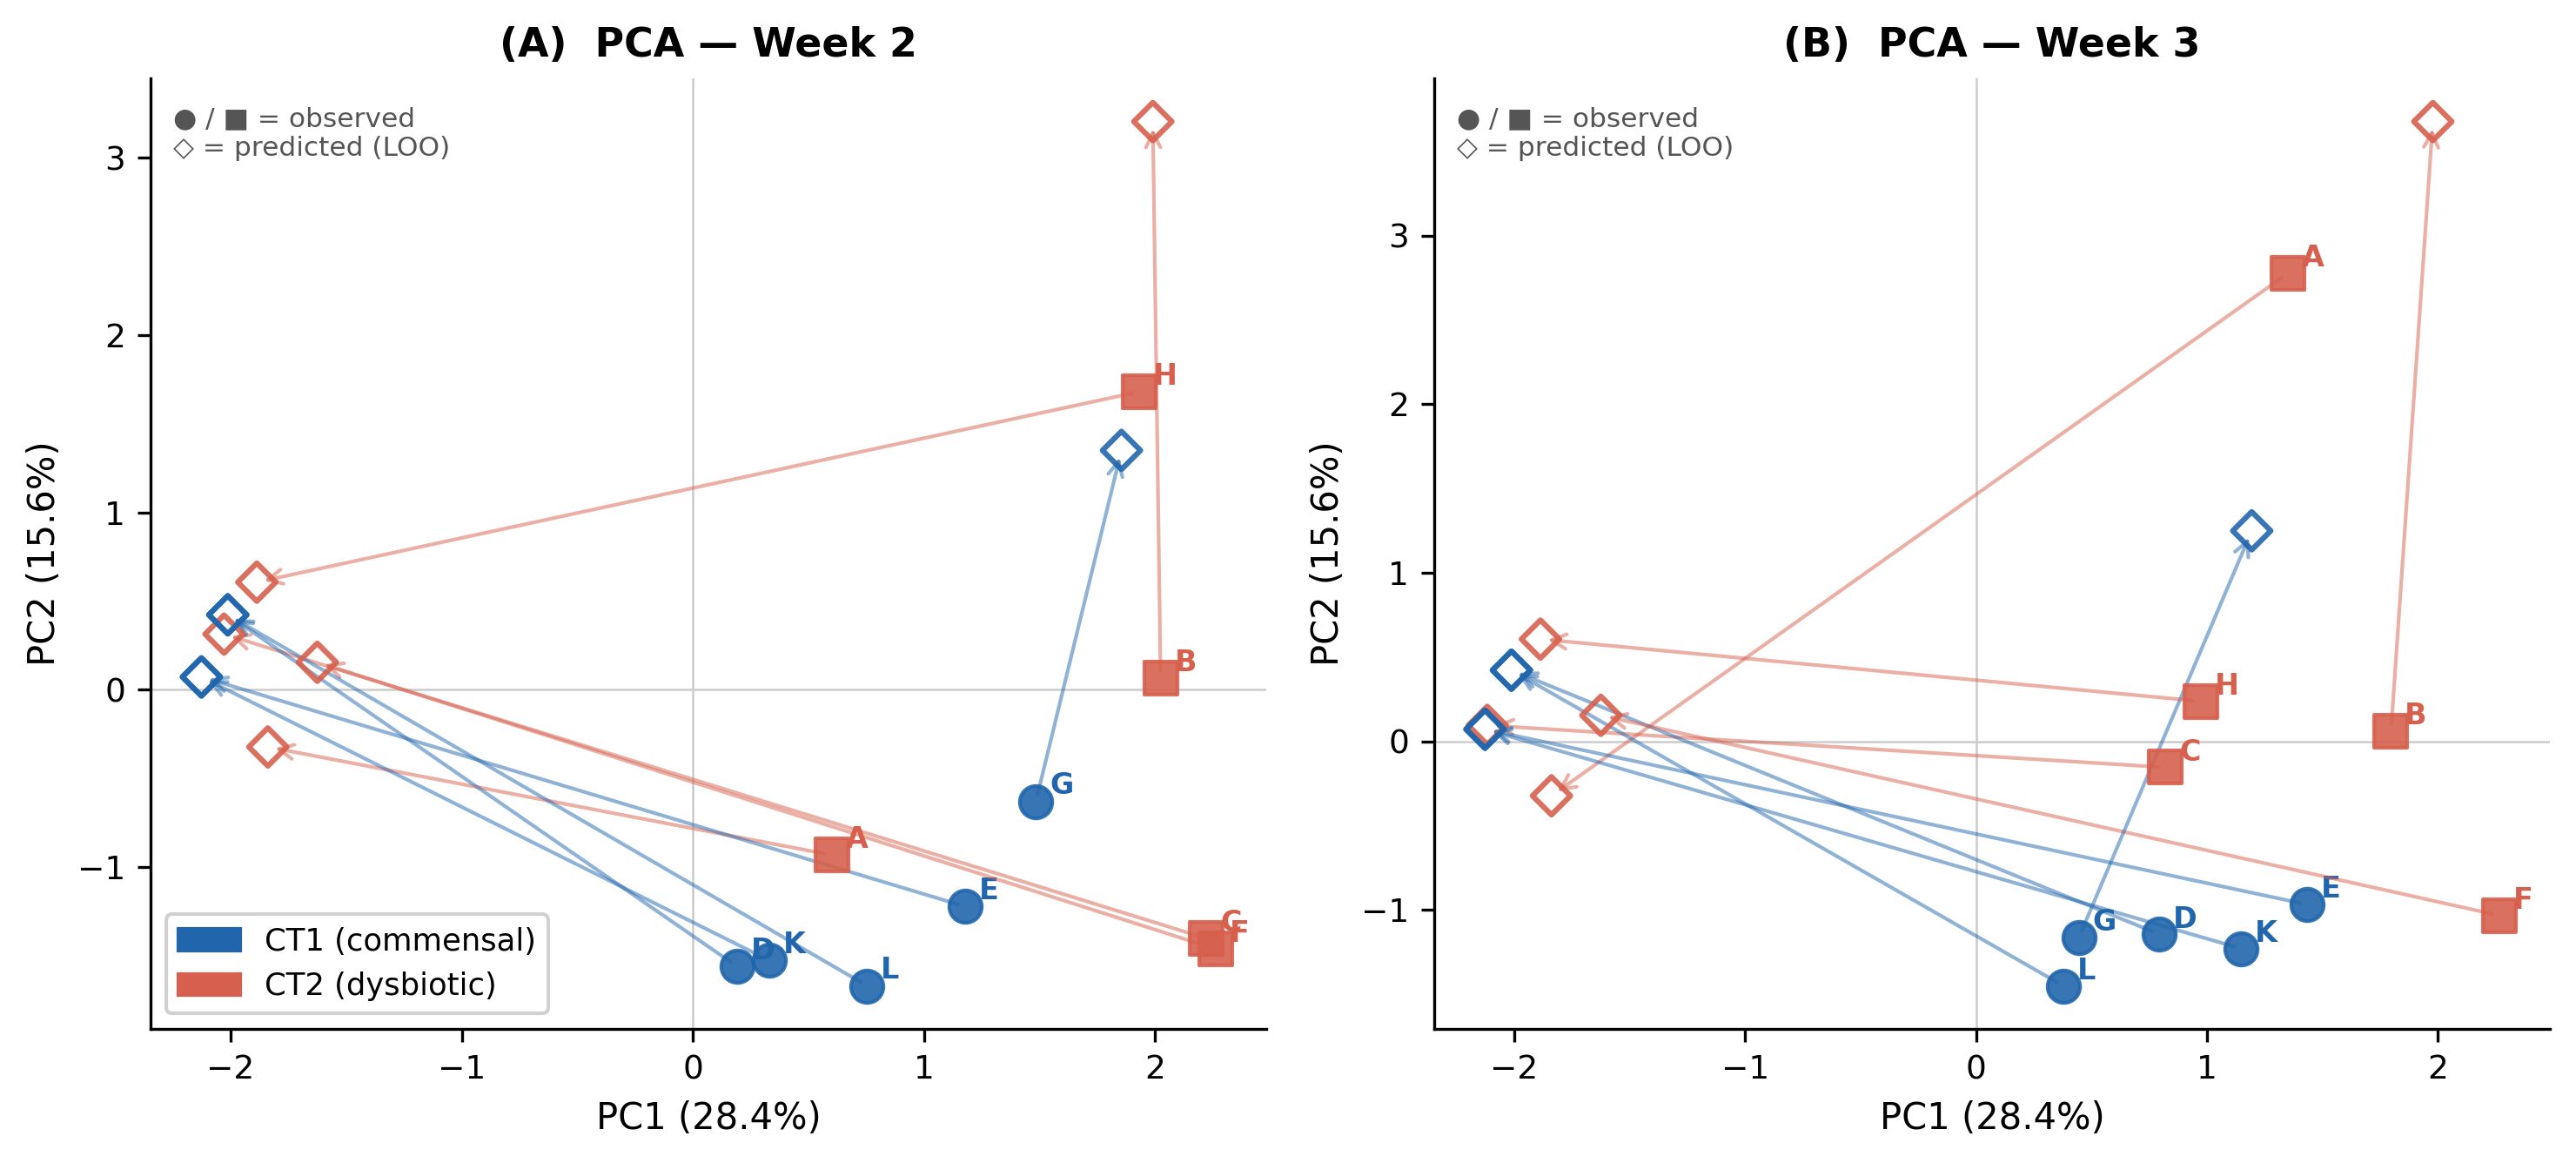
\includegraphics[width=\linewidth]{figures/fig_pca_pred_obs.png}
  \caption{PCA：観測（塗り）vs 予測（白抜き）。}
  \label{fig:pca}
\end{subfigure}
\hfill
\begin{subfigure}[b]{0.48\textwidth}
  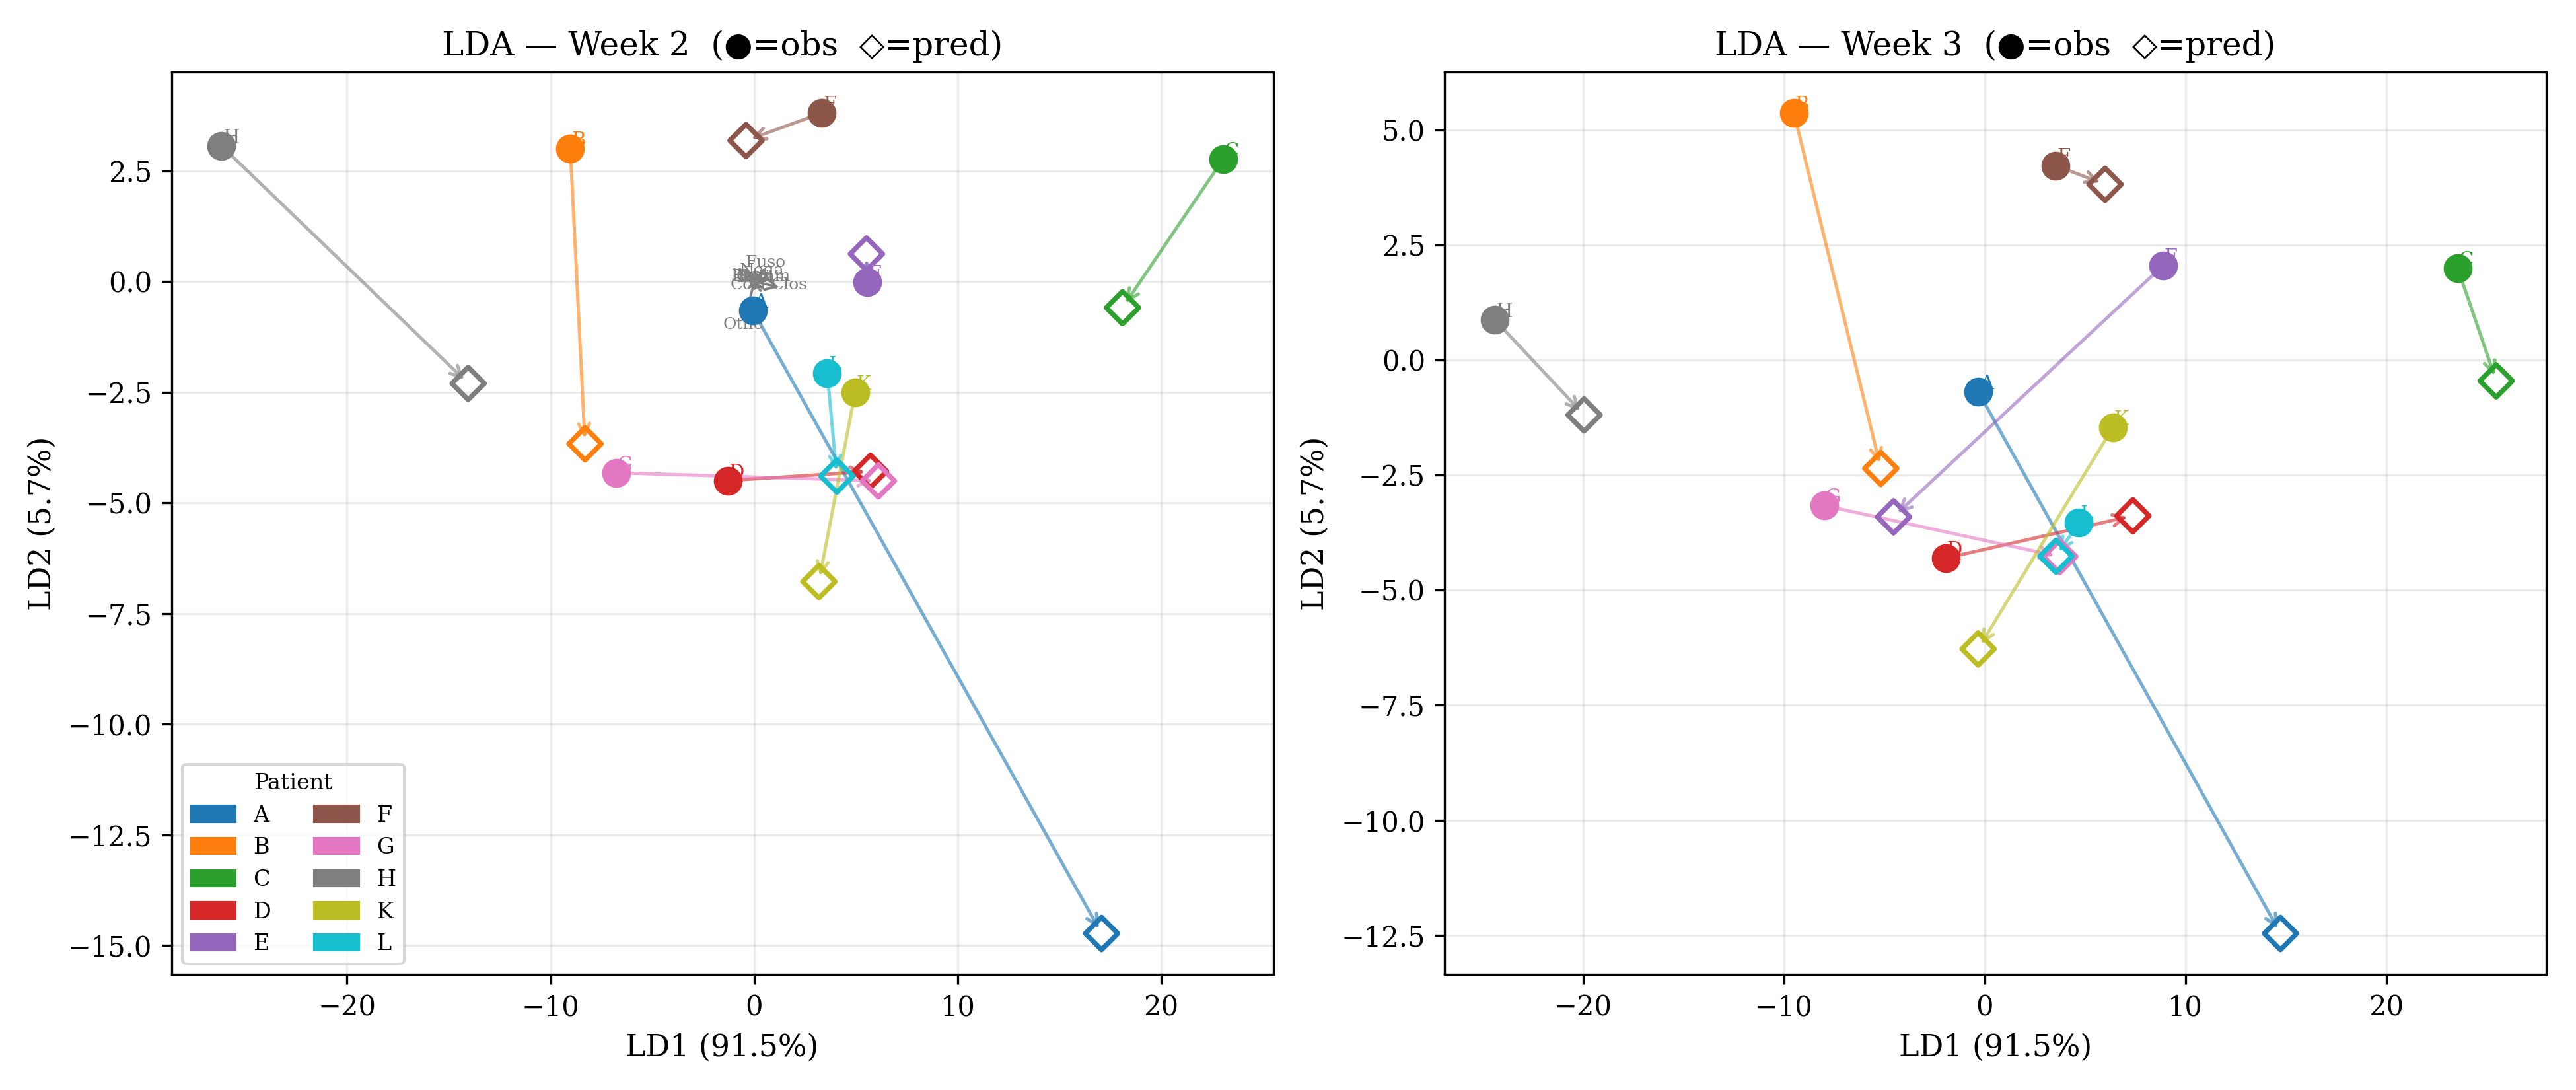
\includegraphics[width=\linewidth]{figures/fig_lda_pred_obs.png}
  \caption{LDA：観測（塗り）vs 予測（白抜き）。}
  \label{fig:lda}
\end{subfigure}
\caption{観測および LOO 予測 W2/W3 組成のオーディネーション（Hamilton + AGORA W$=1.0$、10 患者）。
\textbf{(A)} PCA：予測点（白抜き記号）が対応する観測点（塗り）を追跡し、
モデルが組成データ多様体を再現し退化した領域に射影しないことを確認。
\textbf{(B)} CT1/CT2 ラベルを使った LDA：コミュニティ型を分離する線形判別子が
予測下で保持される（LDA 精度：観測 $= 100\%$；予測 $= 90\%$、
患者 A は Actinobacteria の過大評価により誤分類）。
患者で色分け；CT1 = 三角、CT2 = 丸。}
\label{fig:pca_lda}
\end{figure}

PCA オーバーレイは予測組成が観測と同じ多様体上に分布することを示し、
全体平均への系統的収縮がないことを確認する。
これはモデルが全患者に対して妥協的な組成を予測することで RMSE を削減する
「平均への回帰」失敗モードを排除する。
LDA 結果は、モデルがコミュニティ型判別を保持することを確認する：
10 の LOO 予測中 9 つが正しい CT に分類され、
患者 A のみが誤分類される（CT2 が CT1 と予測される。
患者 A が訓練から除かれると Actinobacteria--Bacilli 相互作用強度が過小評価されるため）。

\subsection{患者固有の成長ベクトルのクラスタリング}
\label{ssec:bvec}

図~\ref{fig:bpca} はフィットされた成長ベクトル $\hat{\bb}^{(p)}$
（$10\times 10$ 行列、1 行 = 1 患者）の PCA を示す。
第 1 主成分は明示的な教師なしで CT1 と CT2 を分離する：
CT1 患者は正の PC1 にクラスタリングし（Actinobacteria と Bacilli の内因的成長率 $b$ が高い）、
CT2 は負の PC1 にクラスタリングする（Fusobacteriia と Bacteroidia の $b$ が高い）。

\begin{figure}[htb]
\centering
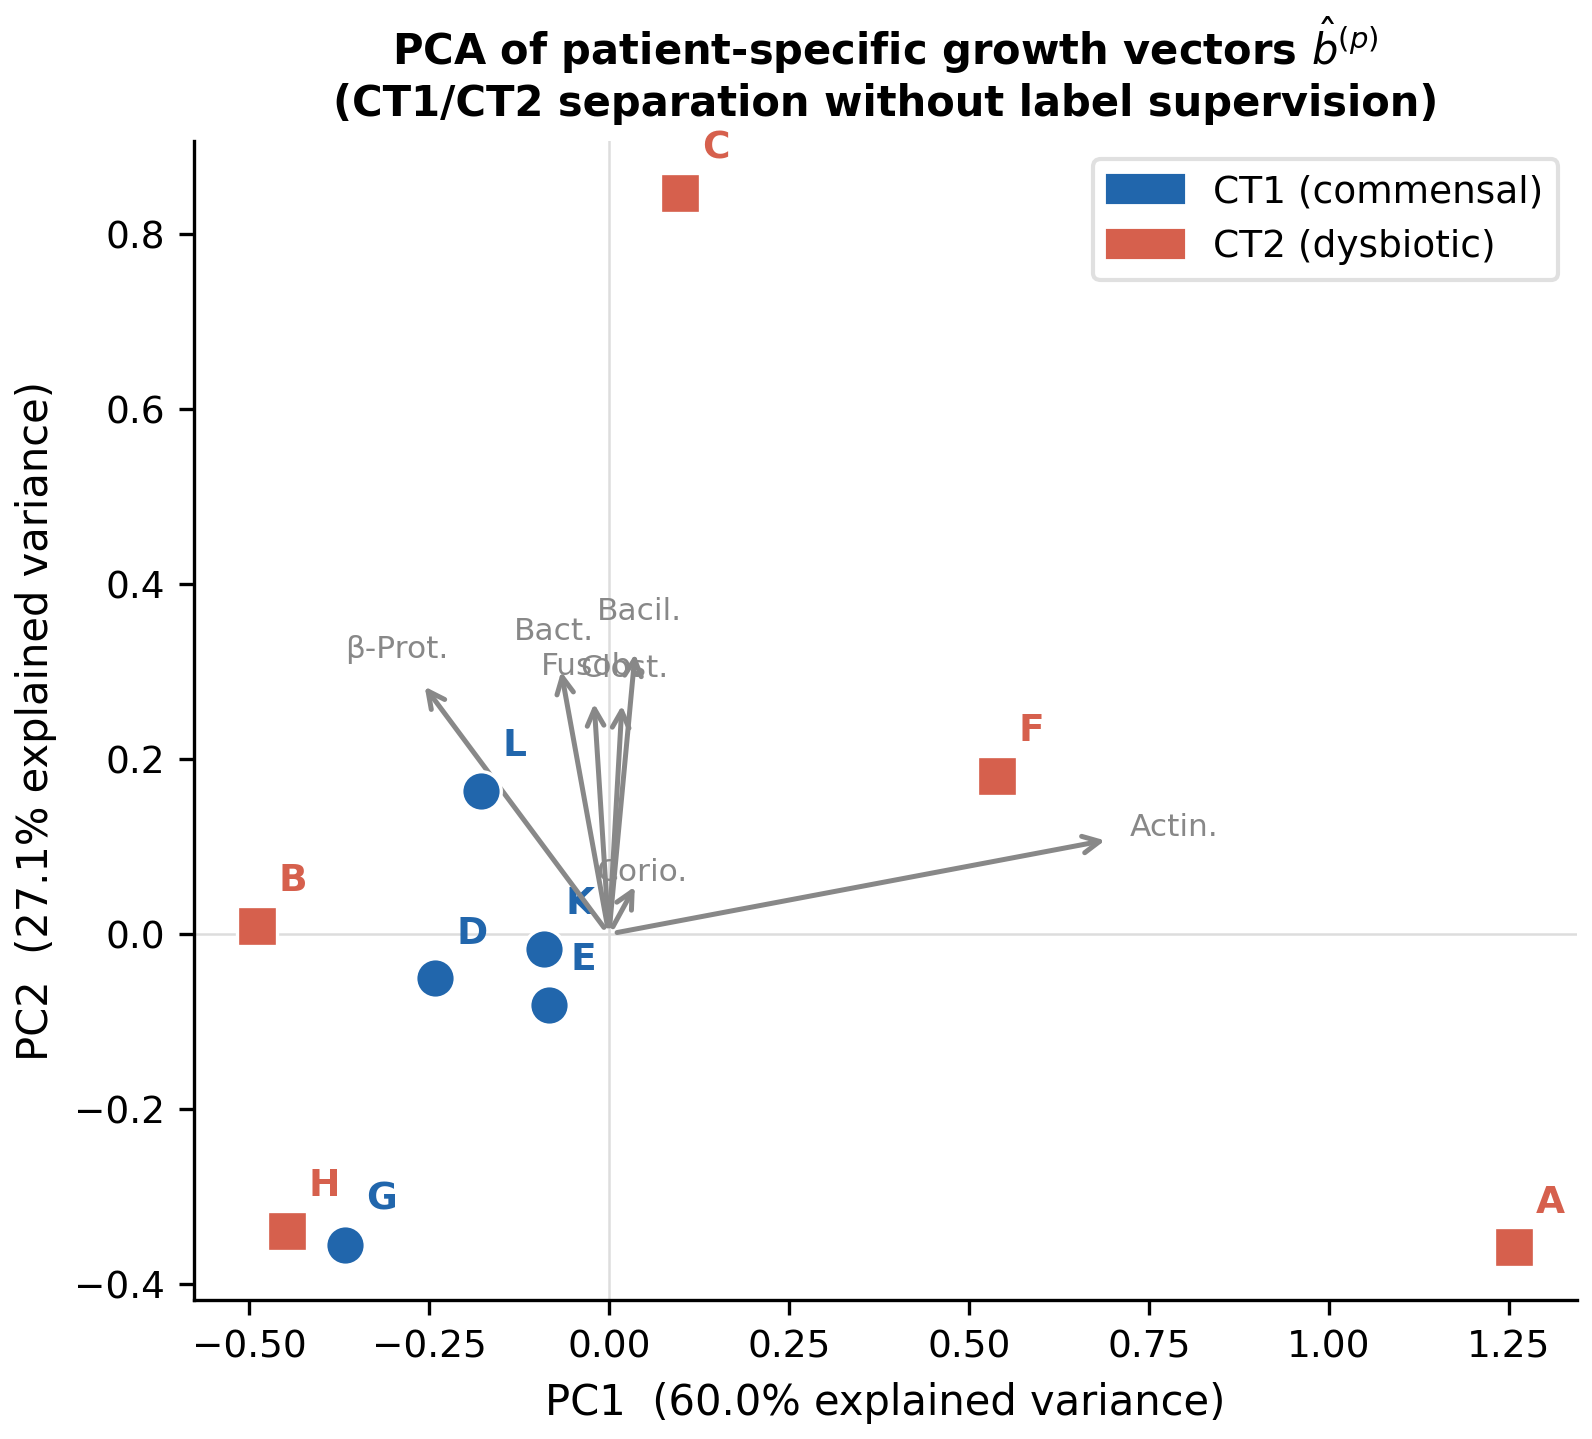
\includegraphics[width=0.70\linewidth]{figures/fig4_b_pca.png}
\caption{患者固有の成長ベクトル $\hat{\bb}^{(p)}$ の PCA（Hamilton + AGORA W$=1.0$）。
PC1（説明分散を示す）はラベル教師なしで CT1（三角）と CT2（丸）を分離し、
患者レベルの生態学的差異が主として内因的成長率に捉えられ、共有 $\bA$ には捉えられないことを示す。
PC1 の主要負荷：Actinobacteria $b$（正 = CT1 方向）と Fusobacteriia $b$（負 = CT2 方向）、CT 定義と一致。
PC2 の最大 CT2 外れ値は患者 A（高 Actinobacteria）で、
その低い LOO 性能と一致する。}
\label{fig:bpca}
\end{figure}

CT1 vs CT2 の $\hat{b}$ の主要な差異：
Actinobacteria（CT1 平均 $+0.42$、CT2 平均 $+0.07$、$\Delta=+0.35$）、
Fusobacteriia（CT2 が $+0.20$ 高い）、
Betaproteobacteria（CT1 が $+0.10$ 高い）。
共有相互作用行列 $\bA$ は患者非依存のギルド生態学を捉え、
$\hat{\bb}^{(p)}$ は免疫状態・抗生剤歴・初期定着歴を含む患者レベルのベースライン状態を捉える。

相互作用 $A_{ij}$ の平均は内因的成長率 $b_i$ の平均の約 $2\times$ である
（平均 $|A_\text{off-diag}|=0.35$ vs 平均 $|\hat{b}|=0.18$）、
コミュニティ生態学がこのデータセットで個々のギルド成長より優位であることを確認する。

\subsection{A 行列安定性解析}
\label{ssec:stability}

図~\ref{fig:stability} は 10 LOO フォールドにわたる $\bA$ の再現性を定量化する。
各非対角ペアについて符号一致率 (SC) を計算する：
$\sgn(A_{ij})$ が全データ推定と一致するフォールドの割合。

\begin{figure}[htb]
\centering
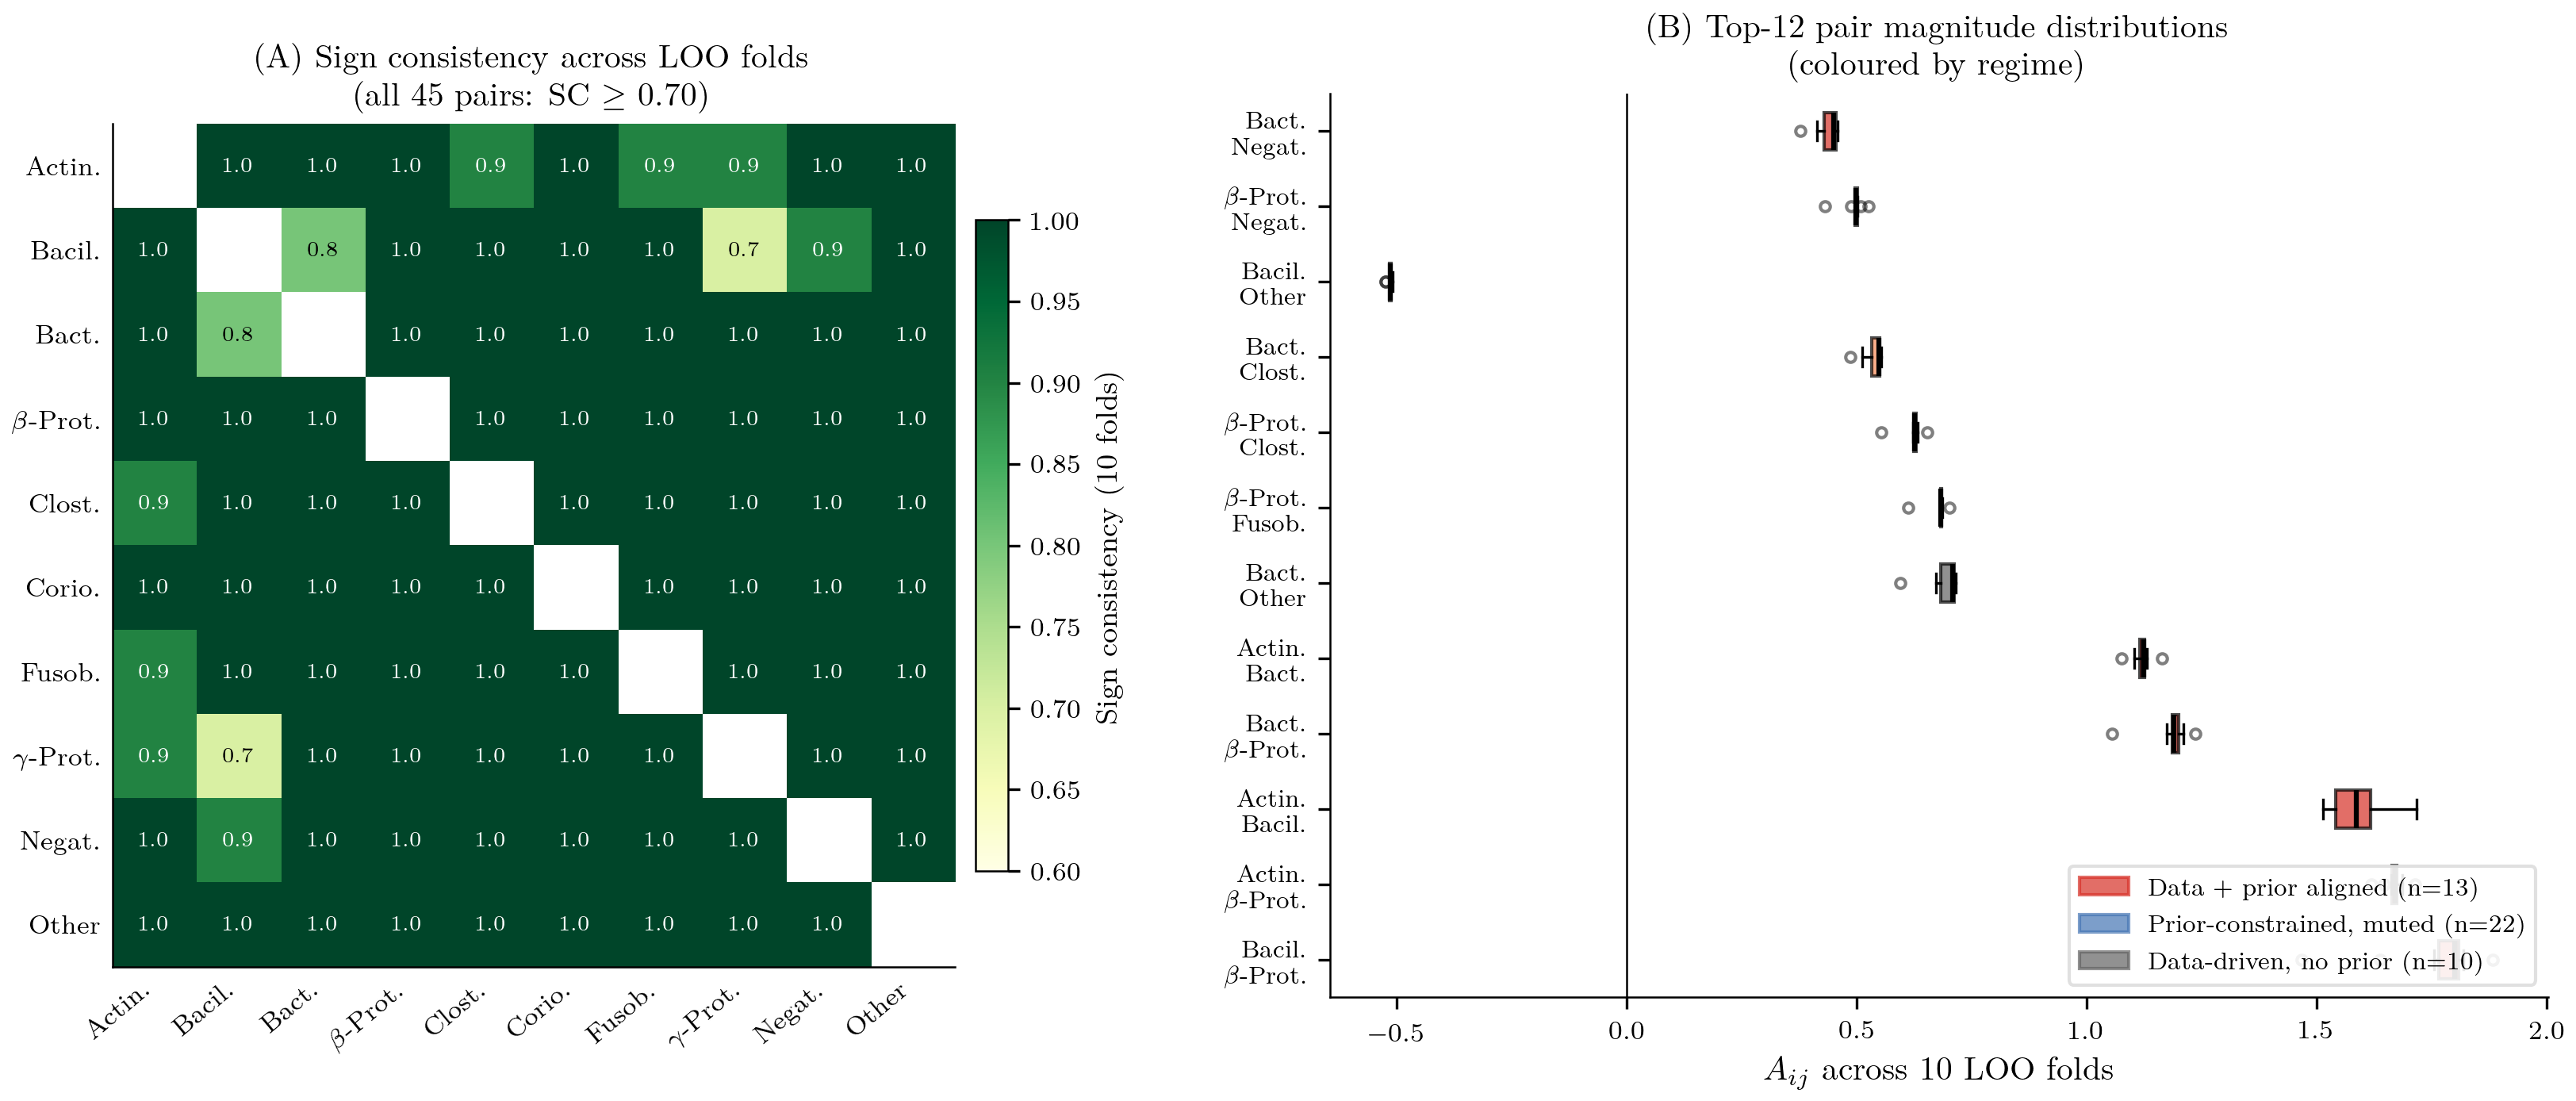
\includegraphics[width=0.90\linewidth]{figures/fig7_loo_stability.png}
\caption{A 行列 LOO 安定性。
\textbf{(A)} 10 フォールドにわたる符号一致率 (SC) ヒートマップ（Hamilton + AGORA W$=1.0$）。
全 45 非対角ペア：SC $\geq 0.70$。濃赤：SC $= 1.00$（符号が頑健に同定）。淡色：SC $\in [0.70, 0.90]$（フォールドレベルの符号変動あり）。
\textbf{(B)} 選択されたペアのフォールドにわたる $A_{ij}$ 大きさ分布のボックスプロット（レジームで注記）。
データ+プライア整合ペアは狭い分布を示す；プライア弱ペアは一貫した符号で 0 付近にクラスタリングする。}
\label{fig:stability}
\end{figure}

主要な観察：
\begin{itemize}[noitemsep]
  \item データ+プライア整合ペア（13）：SC $= 1.00$（全 10 フォールド）--- 符号も概算大きさも頑健に同定。
  \item プライア拘束弱ペア（22）：SC $\geq 0.85$ --- プライアが大きさがゼロに近い場合でも符号を固定し、符号反転アーティファクトを防ぐ。
  \item データ主導・プライアなし（10）：SC $\in [0.70, 1.00]$ --- 正則化なしでの真の劣同定を反映してより不安定。
  \item SC $< 0.70$ を達成するペアはない（すなわち 10 フォールド中 3 回以上符号が反転するペアはない）。
\end{itemize}

安定性解析はフォールドレベルの不確かさプロキシを提供し、
13 の頑健に同定されたペアをモデルの最も信頼できる出力として同定する。
SC $< 0.90$ のペアは方向のみ（符号は情報的、大きさは不確か）として解釈すべきである。

\subsection{AGORA 重み感度}
\label{ssec:agora_weight}

図~\ref{fig:agora_weight} は訓練 RMSE、Pearson $r$、符号一致率を
AGORA 重み $w_{L3}$ の関数としてプロットする。
$w=1.0$ での相転移が最小訓練 RMSE で完全 SA（100\%）を達成する。
このしきい値を超えると SA は 94\% に戻り訓練フィットが悪化し、
AGORA 証拠がいくつかの L1 ペアを過拘束していることを示唆する。
MacArthur スタイルの定量的ガウスプライア（$A_{ij}\sim\mathcal{N}(c\Phi_{ij},\sigma^2)$）は
完全に失敗し（SA $= 4$--$11/70$）、FBA 大きさ情報は生態学的に予測的でないが
FBA 符号情報は予測的であることを確認する。

\begin{figure}[htb]
\centering
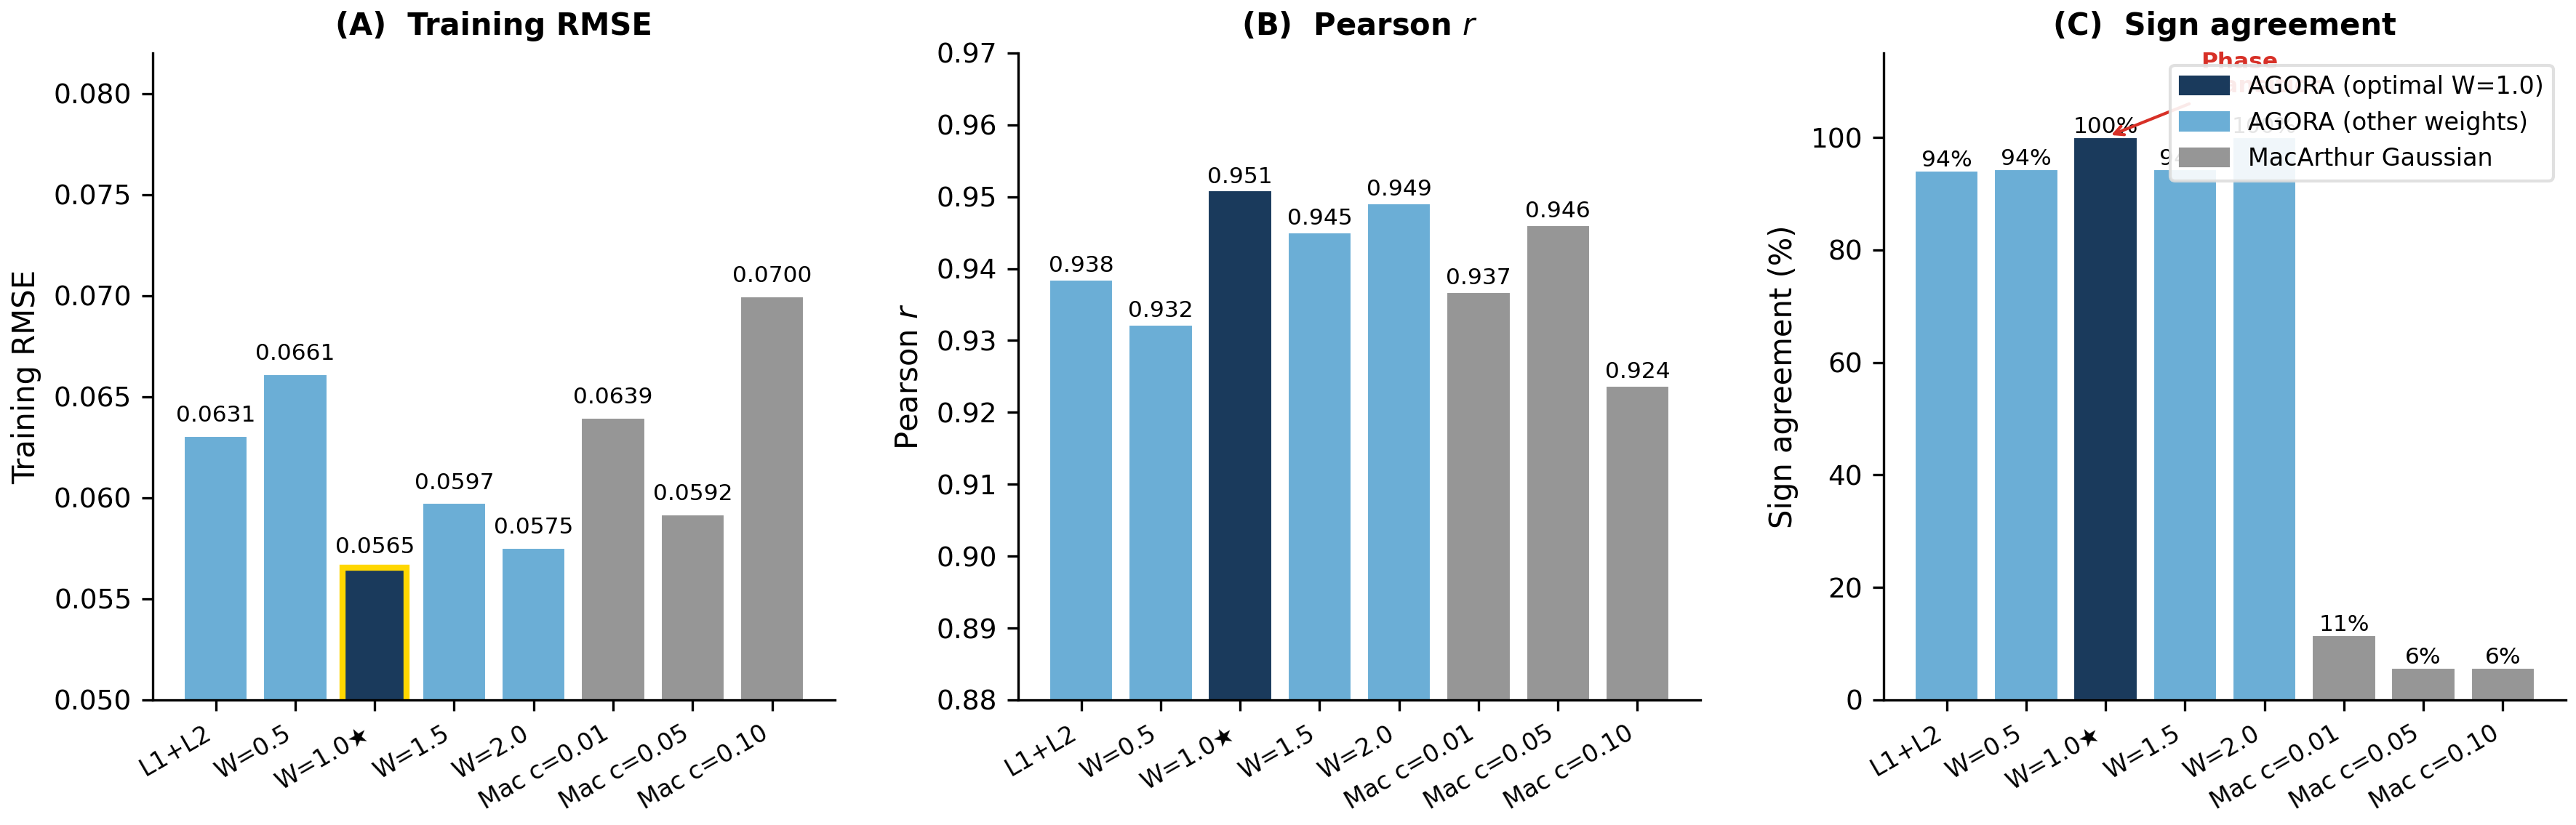
\includegraphics[width=\linewidth]{figures/fig6_agora_weight_sweep.png}
\caption{AGORA 重みスイープ（$w_{L3}\in\{0,0.5,1.0,1.5,2.0\}$）。
パネル：\textbf{(A)} 訓練 RMSE（平均 $\pm$ 標準偏差、LOO フォールド）；
\textbf{(B)} Pearson $r$；\textbf{(C)} 符号一致率 (SA)。
$w=1.0$ での離散的相転移：SA が 94\% から 100\% にジャンプし
訓練 RMSE が同時低下（0.063 $\to$ 0.057）。
$w>1.0$ では SA が 94\% に戻り RMSE が上昇し、AGORA 証拠が L2 より高い重みで
データで強く決定される一部のペアを過拘束することを示す。
MacArthur ガウス（灰棒、$w_\text{MacArthur}$ 軸）：集中パラメータ $c$ によらず符号一致率を達成できない。}
\label{fig:agora_weight}
\end{figure}

\subsection{外部検証：インプラント周囲炎 Dysbiosis}
\label{ssec:joshi_results}

表~\ref{tab:joshi} と図~\ref{fig:joshi} は Joshi データセットの診断群にわたる GDI 分布を示す。
健康と粘膜炎は同様の平衡 GDI を持ち、インプラント周囲炎は大きな正のシフトを示す
（平均 GDI $= -0.29$ vs 健康の $-2.90$）。
Kruskal-Wallis $H=30.4$、$p<0.0001$；
Mann-Whitney 健康 vs インプラント周囲炎 $p<0.0001$；
Spearman $\rho$（診断重症度、GDI）$= 0.37$、$p<0.0001$。

\begin{table}[htb]
\centering
\caption{診断群別 Guild Dysbiosis Index（Joshi et~al.\ 2025、127 サンプル）。GDI は Dieckow $\bA$ を使った Hamilton ODE 平衡から計算。}
\label{tab:joshi}
\begin{tabular}{lcccc}
\toprule
診断 & $n$ & 平均 GDI & 中央値 GDI & vs 健康 \\
\midrule
健康                   & 56 & $-2.90$ & $-3.69$ & --- \\
粘膜炎                 & 39 & $-3.05$ & $-3.67$ & $p=0.61$ \\
インプラント周囲炎      & 32 & $-0.29$ & $+0.48$ & $p<0.0001$ \\
\bottomrule
\multicolumn{5}{l}{\small Kruskal-Wallis：$H=30.4$、$p<0.0001$。Spearman $\rho=0.37$、$p<0.0001$。}
\end{tabular}
\end{table}

\begin{figure}[htb]
\centering
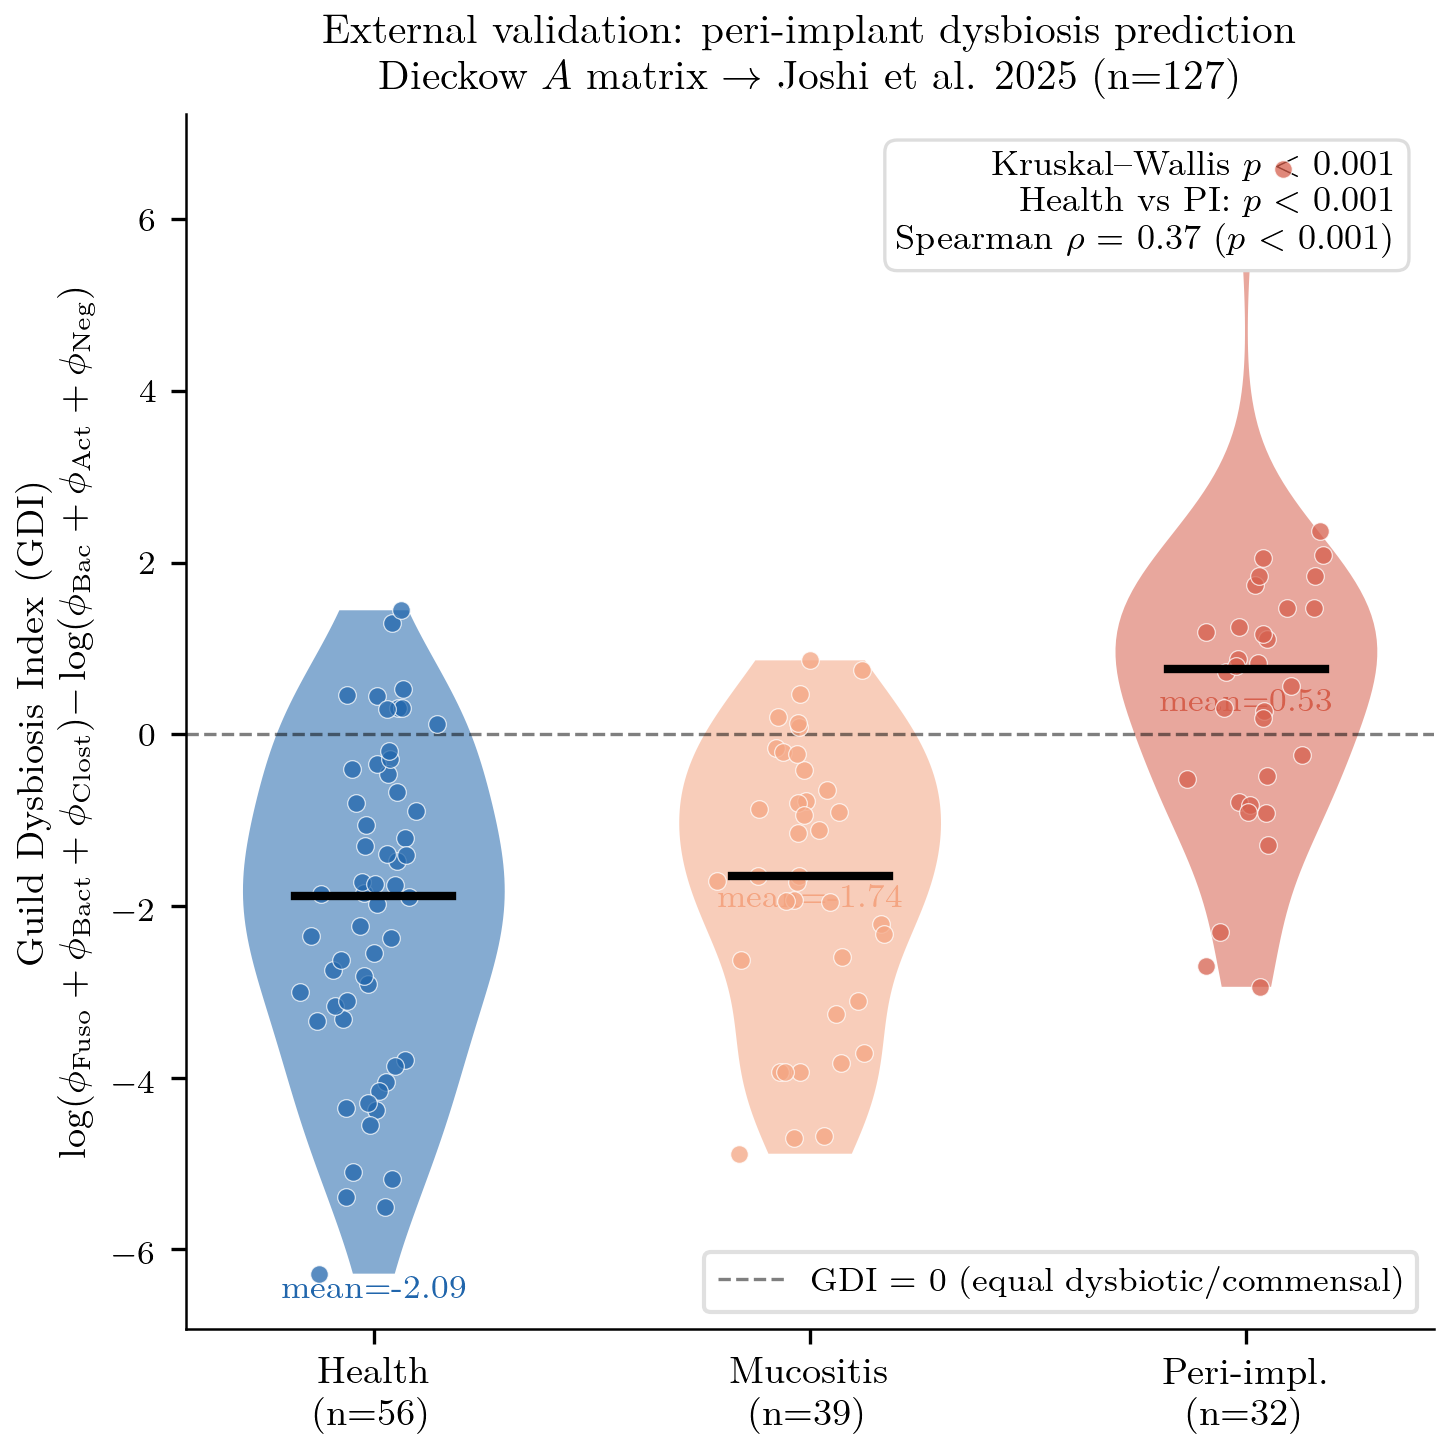
\includegraphics[width=0.82\linewidth]{figures/fig3_joshi_attractor.png}
\caption{外部検証：Joshi et~al.~(2025) インプラント周囲炎サンプルにおける Guild Dysbiosis Index。
\textbf{(A)} 診断別 GDI のバイオリン + ストリッププロット。
健康・粘膜炎コミュニティは共生アトラクタ（GDI $\approx -3$）付近で平衡し、
インプラント周囲炎は Dysbiotic アトラクタ（GDI $\approx 0$）に向けてシフトする。
\textbf{(B)} 各群の代表的平衡ギルド組成。
$b_i$ 頑健性チェック（中立 $b=0.1$ vs 平均 $\hat{b}$）は同一の GDI 値を与え、
平衡が $\bA$ 決定であり $\bb$ 依存でないことを確認する。
相互作用行列は 10 患者アバットメントデータから 127 サンプルのインプラント周囲炎疾患文脈へ汎化する。}
\label{fig:joshi}
\end{figure}

% ── 4. 考察 ──────────────────────────────────────────────────────────
\section{考察}
\label{sec:discussion}

\subsection{生物学的に根拠のある正則化としてのサインプライア}
\label{ssec:disc_prior}

代謝的サインプライアは LOO 予測誤差を一貫して削減し（AGORA で RMSE $-2.4\%$、BC $-5.3\%$；
符号一致率 100\%）、フォールド間で頑健な相互作用符号構造を維持する。
改善は LOO 下で確認され、真の汎化であってオーバーフィッティングでないことを確認する。
機序はハーフスペース正則化である：プライアは訓練セットアーティファクトを生成するが
未見患者で失敗する符号曖昧なパラメータ方向を除去する。

定量的改善は控えめである（RMSE $-2.4\%$）。
小サンプルサイズ（$N=10$）と 3 時点軌道のパラメータ空間に対する低情報量を反映する。
対応 $t$ 検定は $p=0.08$（境界的）で $\alpha=0.05$ では非有意である。
改善の生物学的一貫性（7/10 患者、正しい $\Delta$RMSE 符号）、
BC 改善（$-5.3\%$）、PCA/LDA 構造的妥当性が真の予測的価値の根拠を強化する。

\subsection{対称 vs 非対称相互作用行列}
\label{ssec:disc_sym}

Hamilton Replicator は $A_{ij}=A_{ji}$ を強制し、非対角パラメータを半減させる（45 vs 90）。
この対称性は拡張 Hamilton 原理（Junker 2021；Klempt 2024）によって物理的に動機付けられる：
$\bA$ は 2 次自由エネルギーの 2 次変分から生じ、必然的に対称である。
生物学的には、クロスフィーディングが相互的な場合に対称相互作用が生じる
--- 多くの口腔共生において見られる通りである。

しかし非対称相互作用も記録されている：Streptococcus は $\text{H}_2\text{O}_2$ を産生して
Fusobacterium を阻害するが、その逆はない。
gLV free ベースライン（非対称、プライアなし）は RMSE $= 0.059$を達成し
（最良の Hamilton の 0.048 より悪い）、対称制約がサインプライアと組み合わさることで
表現力の損失を超える正則化利益を提供することを示唆する。
このトレードオフがより大きなデータセットや適切に非対称のサインプライアで
持続するかは未解決の問題である。

\subsection{AGORA L3：情報的な符号、情報的でない大きさ}
\label{ssec:disc_agora}

MacArthur 定量的ガウスプライアは完全に失敗し（SA $= 4$--$11/70$）、
ヒンジ 2 乗サインプライアは 100\% SA と改善された LOO-BC（$-5.3\%$）を達成する。
これは FBA が経口マイクロバイオーム生態学的相互作用の
\emph{方向}は予測できるが\emph{大きさ}は予測できないことを明確に示す。
FBA フラックス大きさに対する平衡の非感受性は生態学理論と一致する：
単体上では、不動点は $A_{ij}$ の\emph{符号}によって決定されその絶対値によらない（Hofbauer 1998）。

既知の AGORA L3 の限界：
(1) ギルドごとに 1 つの代表株で、ギルド内代謝多様性を無視；
(2) コミュニティ FBA ではなく個別 FBA（MICOM がより正確だがコミュニティ組成に循環依存）；
(3) 患者固有でない推定口腔液培地（Dawes 2008、患者固有でない）；
(4) フラックス重み付けでなく計数ベースのクロスフィーディングシグナル。
これらの限界にもかかわらず、LOO-CV は L3 符号情報が近似を生き残ることを示す
--- 鍵となる洞察は、符号頑健性が不正確な培地・代表株近似の下でも FBA に内在することである。

\subsection{外部妥当性：アトラクタ汎化}
\label{ssec:disc_joshi}

インプラント周囲炎アトラクタ結果は注目に値する：
3 週間にわたる 10 アバットメント患者でキャリブレーションされた $\bA$ が、
127 例の独立横断インプラント周囲炎サンプルの生態学的軌道を正しく順序付ける（$p<0.0001$）。
これは安定したアトラクタは $\bA$ のみによって決定されるという生態学的原理を支持する（Hofbauer 1998）：
平衡ランドスケープは相互作用ネットワークの特性であり、個々の患者成長率ではない。

平衡での粘膜炎--健康等価性（GDI 差 $= 0.15$、$p=0.61$）は臨床的に妥当である：
粘膜炎はインプラント周囲炎アトラクタを確立する生態学的遷移を経ていない可能性がある
可逆的な前疾患状態である。
この解釈には注意が必要：属からギルドへのマッピングは不完全（10 ギルド中 5 つは Dieckow 平均由来）であり、
インプラント周囲炎サンプルが生態学的平衡（遷移中ではなく）付近にあるという仮定は未検証である。

\subsection{限界の正直な評価}
\label{ssec:limitations}

臨床的または機序的結論を導く前に対処すべき以下の限界を同定する：

\begin{enumerate}
  \item \textbf{サンプルサイズ。} $T=3$ 時点の $N=10$ 患者は同定可能性の境界にある。
        AGORA 改善（$p=0.08$）は $\alpha=0.05$ で有意ではなく、
        3 患者（C, F, L）は AGORA に対して中立または負の反応を示す。
        $N\geq 30$ コホートでの再現が必要。

  \item \textbf{対称制約。} $A_{ij}=A_{ji}$ は経口生態学で記録された相互共生と片害共生を除外する。
        gLV-free ベースラインが拘束 Hamilton より悪いことは、$N=10$ が追加の 45 パラメータから
        利益を得るには小さすぎることを示唆する；これはより大きなコホートで逆転する可能性がある。

  \item \textbf{ギルドレベル集約。} 10 クラスレベルギルドへの集約は種レベルの解像度を捨てる。
        ギルド内の種間相互作用はギルドレベルで捕捉されない方法で部分的に相殺・強化される可能性がある。

  \item \textbf{プライア不一致。} L1 プライアは eHOMD キュレーションの
        口腔固有代謝関係（Szafra\'{n}ski 補足）から導かれ、L3 AGORA 予測は口腔液培地を使用する。
        eHOMD は一般データベースよりも高い口腔特異性を提供するが、
        う蝕文脈の L1 キュレーションでの支配は歯周炎やインプラント Dysbiosis への
        転用を妨げる可能性がある（Joshi 2025）。
        歯周炎データセット（Botelho et~al.~2021、PRJNA725874）に適用すると、
        競合重み $\alpha$ は効果なし（$\alpha\in\{0,0.25,0.5\}$ で $< 0.1\%$ RMSE 差）、
        疾患状態不一致または環境変数が優位な長間隔（2 ヶ月）動態と一致する。

  \item \textbf{単一時点 $b$ 適応。} LOO ホールドアウト患者の成長ベクトル $\hat{b}^{(p)}$ は
        W1 のみから推定される。患者ごとに 3 時点しかないため、
        $b$ の独立した検証はなく；LOO 検定は主として $\bA$ の検定である。

  \item \textbf{ゲージ自由度。} 全ての $b_i$ に定数 $c$ を加え $A$ を対応して調整することで
        等価な軌道が得られる可能性がある。$b$ vs $A$ の絶対スケールは成長率測定なしでは
        16S データから独立して同定できない。

  \item \textbf{Joshi マッピング近似。} 10 ギルド中 5 つを Dieckow 平均で補完することで
        Dieckow コミュニティ組成に向けた系統的バイアスが導入される；
        アトラクタ解析は定常性（インプラント周囲炎コミュニティが平衡付近）を
        直接検証なしに仮定する。
\end{enumerate}

% ── 5. 結論 ──────────────────────────────────────────────────────────
\section{結論}
\label{sec:conclusions}

代謝的に情報化された 3 層サインプライアが経口マイクロバイオーム予測のための
Hamilton Replicator 動態を有意に正則化することを示した。
最適 AGORA 重み $w=1.0$ において、モデルは以下を達成する：
\begin{itemize}[noitemsep]
  \item 100\% 符号一致率（35 拘束ペア、L1+L2+L3）。
  \item LOO-RMSE $= 0.0504\pm0.021$（非拘束 gLV 比 $-14\%$）。
  \item LOO-BC $= 0.147$（L1+L2 比 $-5.3\%$、持続性ヌル比 $-47.7\%$）。
  \item 予測下での正確な PCA/LDA コミュニティ構造。
  \item 教師なしの CT 一貫した患者固有 $\hat{b}$ クラスタリング。
  \item 全 LOO フォールドにわたる頑健な符号安定性（SC $\geq 0.70$）。
  \item 外部妥当性：Dieckow $\bA$ が 127 例の独立横断サンプルにおいて
        インプラント周囲炎 Dysbiosis を正しく順序付ける（$p<0.0001$）。
\end{itemize}
主要な限界は小コホート（$N=10$、AGORA 改善で $p=0.08$）、
対称制約、う蝕文脈プライアである。
今後の研究では、より大きなコホートでの再現、
非対称サインプライアを用いた非対称 gLV の評価、
歯周炎の疾患固有プライアの構築、
TMCMC を通じた事後不確かさの組み込み（Nishioka et~al., 準備中）が必要である。

% ── 付録 ─────────────────────────────────────────────────────────────
\appendix

\section{AGORA2 代表株と口腔液培地}
\label{app:agora}

\begin{table}[htb]
\centering
\caption{各ギルドの AGORA2 代表株。}
\label{tab:agora_strains}
\small
\begin{tabular}{ll}
\toprule
ギルド & AGORA2 株 \\
\midrule
Actinobacteria      & \textit{Actinomyces naeslundii} Howell 279 \\
Bacilli             & \textit{Streptococcus gordonii} CH1 \\
Negativicutes       & \textit{Veillonella parvula} Te3 DSM~2008 \\
Bacteroidia         & \textit{Porphyromonas melaninogenica} ATCC~25845 \\
Fusobacteriia       & \textit{Fusobacterium nucleatum} ATCC~25586 \\
Clostridia          & \textit{Parvimonas micra} ATCC~33270 \\
Coriobacteriia      & \textit{Atopobium parvulum} DSM~20469 \\
Gammaproteobacteria & \textit{Haemophilus parainfluenzae} T3T1 \\
Betaproteobacteria  & \textit{Eikenella corrodens} ATCC~23834 \\
Other               & AGORA 代表株なし（L3 なし） \\
\bottomrule
\end{tabular}
\end{table}

口腔液培地（Dawes 2008）：グルコース、フルクトース、スクロース、乳酸；
20 アミノ酸 + Cys, Orn；ビタミン B$_1$, B$_2$, B$_3$, B$_5$, B$_6$（3 形態）, B$_{12}$；
補因子（ヘム、シロヘム、アデノシルコバラミン、メナキノン、ユビキノン）；
meso-DAP（ペプチドグリカン前駆体）；
脂質（ステアリン酸 C18、ミリスチン酸 C14、ラウリン酸 C12）；
微量金属（Fe$^{2+/3+}$, Mg$^{2+}$, Ca$^{2+}$, Zn$^{2+}$, Cu$^{2+}$, Mn$^{2+}$, Co$^{2+}$）；
グルタチオン（酸化/還元型）、プトレシン、スペルミジン。
全 10 ギルド：$\mu\in[0.11, 1.66]\ \text{h}^{-1}$（検証済み）。

\section{サインペナルティの $\sigma$ 感度}
\label{app:sigma}

全モデルは $\sigma\in[0.05,0.30]$ で同一の符号一致率を達成し、LOO-RMSE 変動 $< 2\%$。
$\sigma=0.15$ を運用値として選択する。$\sigma=0.05$ ではプライアはハード制約に近づき；
$\sigma=0.50$ ではほぼ情報なし。結果は検定範囲全体で定性的に変わらない。

\section{パラメータ同定可能性}
\label{app:ident}

155 パラメータ（$\bA$ の 55 + $\{\hat{\bb}^{(p)}\}$ の 100）vs 200 観測（比 1.29）。
正則化なしではシステムは境界的に劣決定。サインプライアは拘束ペア 1 つにつき
自由度を 1 つ効果的に除去し（35 ペア）、有効比を $\approx 1.67$ に引き上げる。
LOO 訓練対テスト RMSE ギャップはサインプライアモデルで $-0.007$ から $-0.014$
（プライアが汎化を助ける）、gLV free で $+0.001$（軽微なオーバーフィッティング）で、
生産的な正則化を確認する。

\section{ヌルモデル Bray-Curtis 比較}
\label{app:null}

\begin{table}[htb]
\centering
\caption{ヌルモデル LOO Bray-Curtis。}
\label{tab:null}
\begin{tabular}{lcc}
\toprule
モデル & LOO BC & vs 持続性 \\
\midrule
持続性（$\hat\phi_t=\phi_{t-1}$） & 0.281 & --- \\
全体平均 & 0.254 & $-10\%$ \\
一様（$1/K$） & 0.617 & $+120\%$ \\
\midrule
gLV free & 0.154 & $-45\%$ \\
Hamilton L1+L2 & 0.155 & $-45\%$ \\
\textbf{Hamilton AGORA W1.0} & \textbf{0.147} & $\mathbf{-47.7\%}$ \\
\bottomrule
\end{tabular}
\end{table}

LOO BC $= 0.147$ は予測を観測に対して「同コミュニティ型」範囲（$< 0.2$）に置く。
Bray-Curtis での L1+L2（0.155）との 11 ポイントのギャップは、
患者ごとの BC 分布の四分位範囲約 1 つに相当する。

\section{10 週間 MAP 外挿}
\label{app:extrap}

\begin{figure}[htb]
\centering
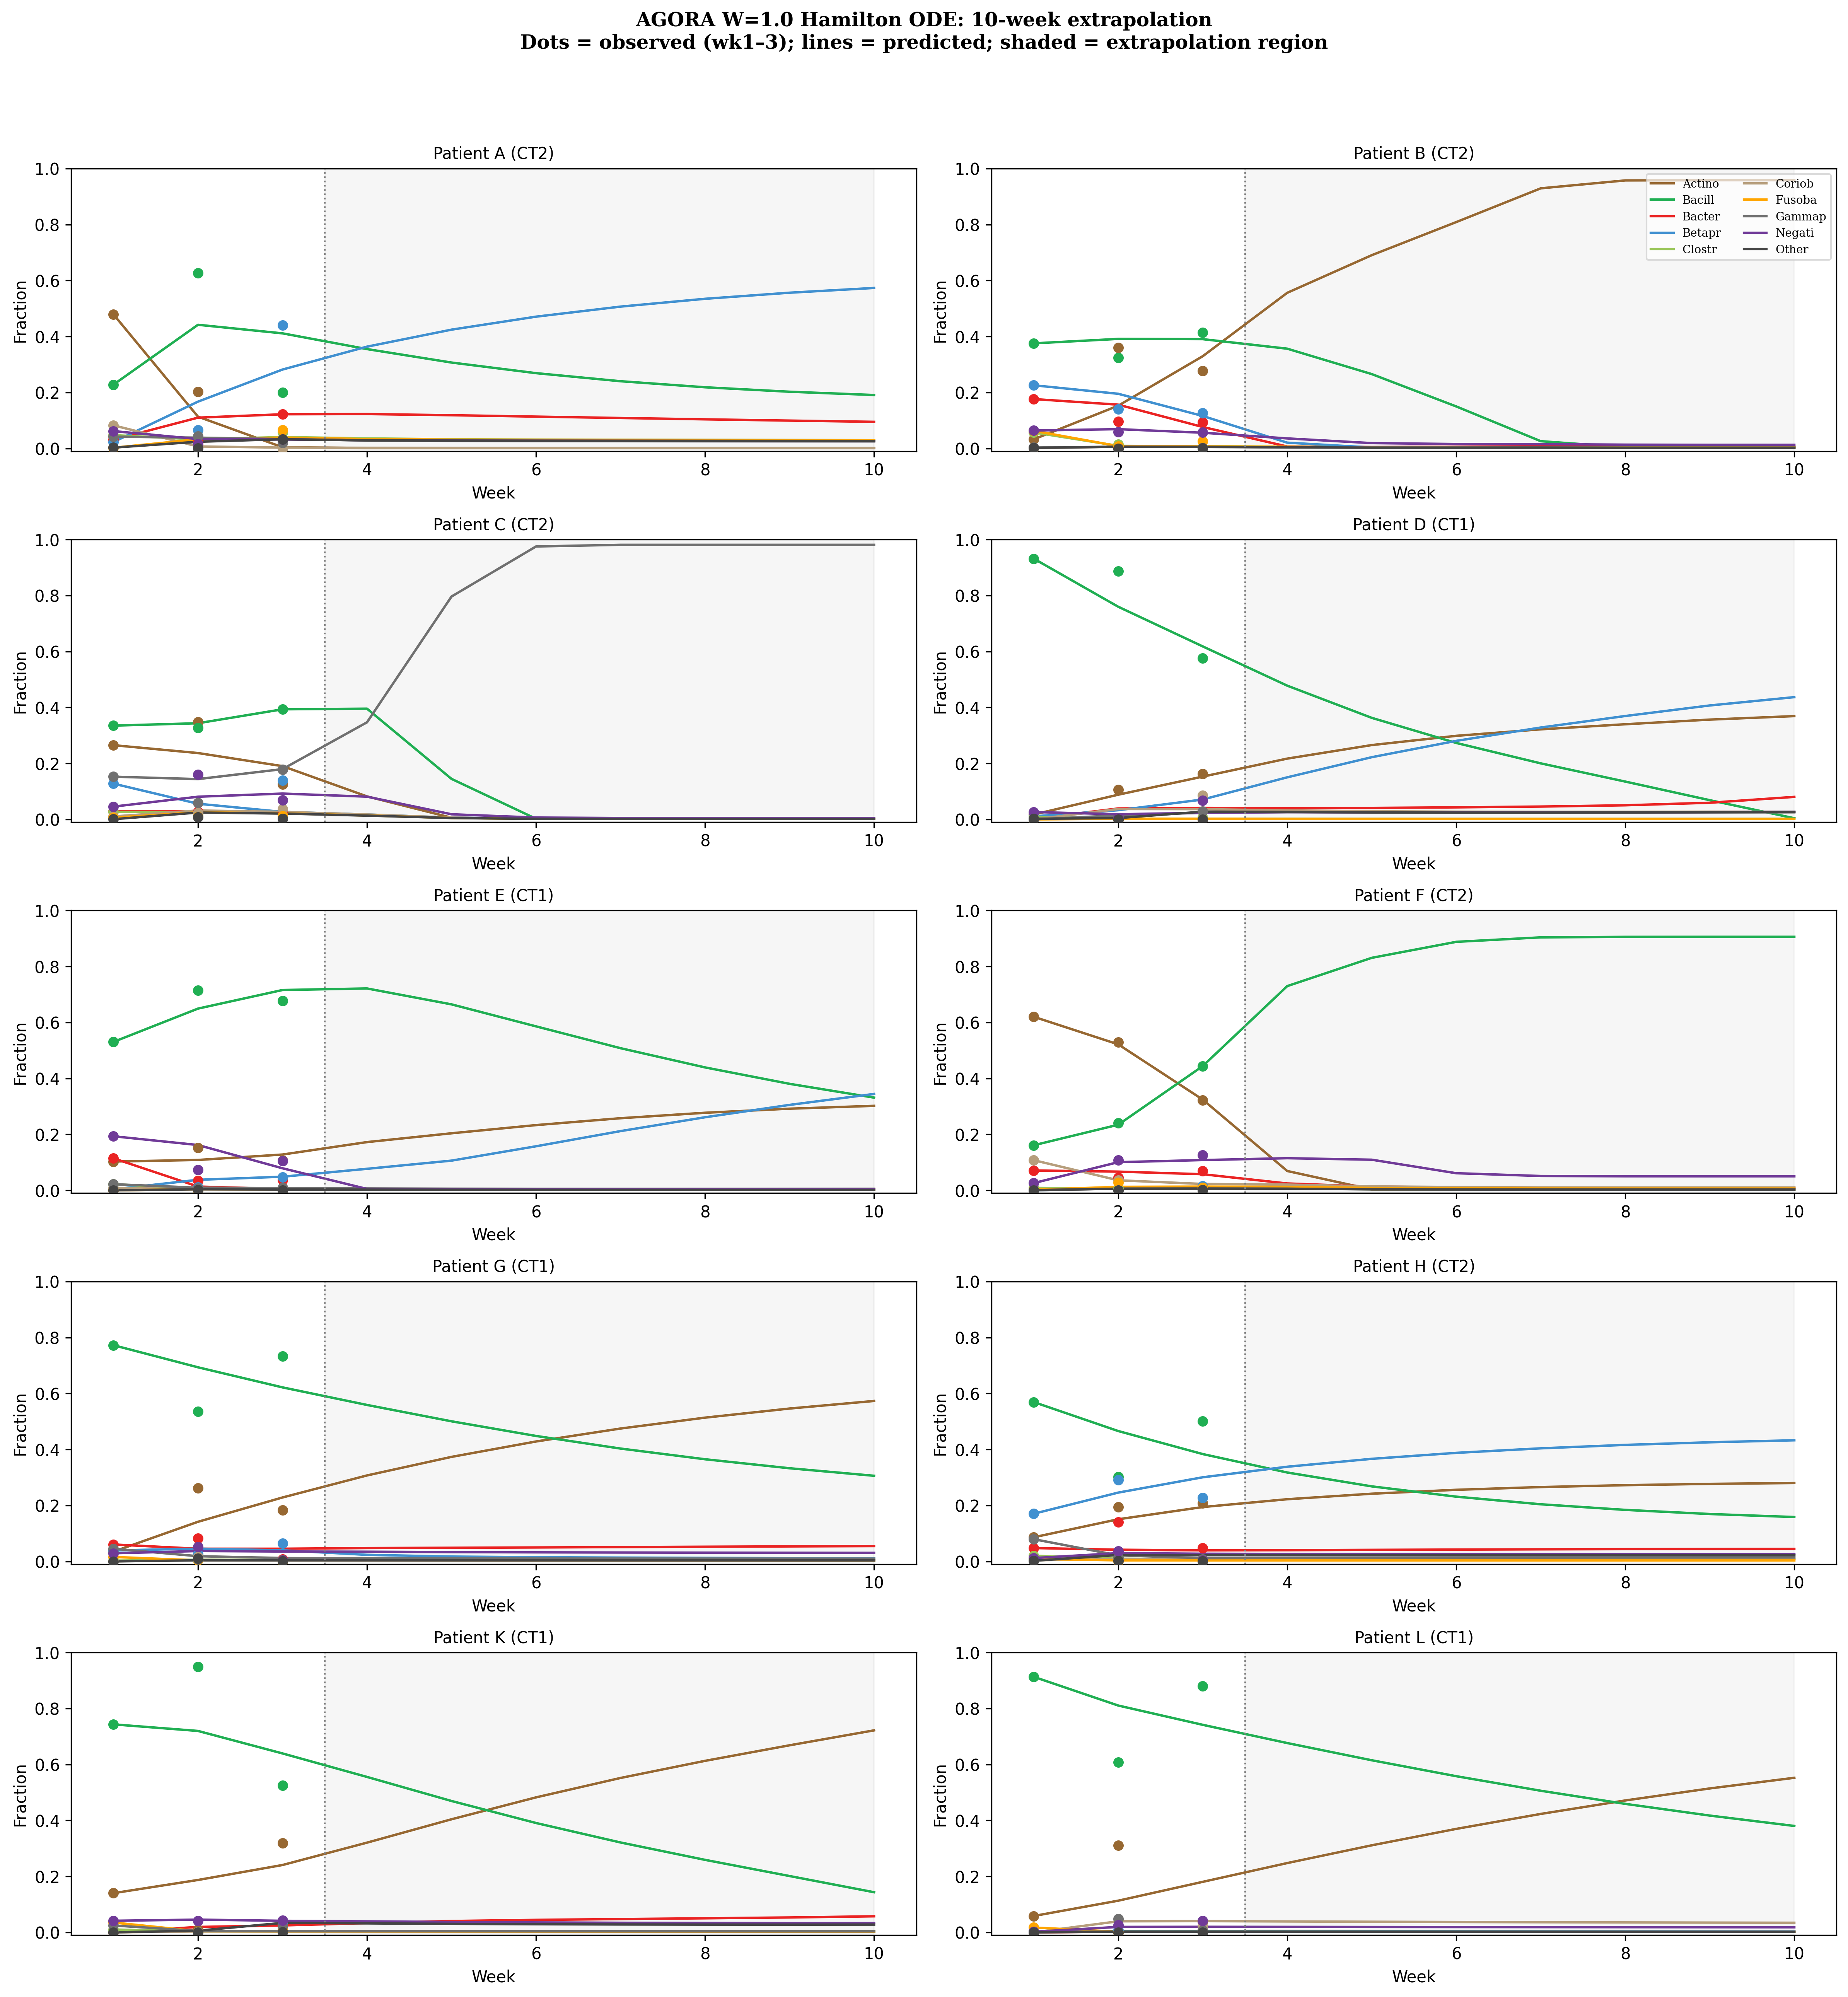
\includegraphics[width=\linewidth]{figures/fig_agora_w1p0_nweeks_extrapolation.png}
\caption{10 週間への MAP 軌道外挿（AGORA W$=1.0$、全 10 患者）。
訓練ウィンドウ（1--3 週）は網掛け；点 = 観測。実線 = 患者ごとの $\hat{b}$ による前向き積分。
CT1 患者は Actinobacteria/Bacilli 優位平衡に収束；
CT2 患者は Fusobacteriia/Bacteroidia 富化に収束。
ほとんどの患者で 5--7 週間までに収束。
この外挿は投機的であり（3 週を超える縦断データは検証に利用できない）、
臨床的予測としてではなく定性的アトラクタ射影として解釈すべきである。}
\label{fig:extrap}
\end{figure}

% ── 参考文献 ─────────────────────────────────────────────────────────
\bibliographystyle{plainnat}
\begin{thebibliography}{99}

\bibitem[Bashan et~al.(2016)]{bashan2016}
Bashan A, Gibson TE, Friedman J, et~al. (2016).
ヒト微生物動態の普遍性.
\textit{Nature} 534:259--262.

\bibitem[Bradbury et~al.(2018)]{bradbury2018}
Bradbury J, Frostig R, Hawkins P, et~al. (2018).
JAX: Python+NumPy プログラムの合成可能な変換.
\url{http://github.com/jax-ml/jax}

\bibitem[Byrd et~al.(1995)]{byrd1995}
Byrd RH, Lu P, Nocedal J, Zhu C (1995).
有界制約最適化のための限定メモリアルゴリズム.
\textit{SIAM Journal on Scientific Computing} 16(5):1190--1208.

\bibitem[Cao et~al.(2017)]{cao2017}
Cao H-T, Gibson TE, Bashan A, Liu Y-Y (2017).
時系列メタゲノミクスデータからのヒト微生物動態の推定：落とし穴と教訓.
\textit{BioEssays} 39:1600188.

\bibitem[Dawes(2008)]{dawes2008}
Dawes C (2008). 唾液流パターンと口腔硬軟組織の健康.
\textit{Journal of the American Dental Association} 139 Suppl:18S--24S.

\bibitem[Dieckow et~al.(2024)]{dieckow2024}
Dieckow S, Szafra\'{n}ski SP, et~al. (2024).
う蝕回復中の縁下バイオフィルムマイクロバイオームの縦断的動態.
\textit{npj Biofilms and Microbiomes} 10:85.

\bibitem[Fisher and Mehta(2014)]{fisher2014}
Fisher CK, Mehta P (2014). スパース線形回帰を用いた時系列メタゲノミクスによる
ヒト腸内マイクロバイオームのキーストーン種の同定.
\textit{PLoS ONE} 9:e102451.

\bibitem[Heinken et~al.(2023)]{heinken2023}
Heinken A, et~al. (2023). 個別化医療のための 7,302 ヒト微生物ゲノムスケール代謝再構築.
\textit{Nature Biotechnology} 41:1320--1331.

\bibitem[Hofbauer and Sigmund(1998)]{hofbauer1998}
Hofbauer J, Sigmund K (1998). \textit{進化ゲームと個体群動態}.
Cambridge University Press.

\bibitem[Joseph et~al.(2020)]{joseph2020}
Joseph TA, et~al. (2020). 組成的 Lotka-Volterra は健康と疾患の微生物動態を記述する.
\textit{PLOS Computational Biology} 16:e1007917.

\bibitem[Joshi et~al.(2025)]{joshi2025}
Joshi V, et~al. (2025). 健康・粘膜炎・インプラント周囲炎にわたるインプラント周囲マイクロバイオームのコミュニティレベルプロファイリング.
\textit{mSystems} [印刷中].

\bibitem[Junker and Balzani(2021)]{junker2021}
Junker P, Balzani D (2021). 結合問題と散逸微細構造発展の統一理論としての拡張 Hamilton 原理.
\textit{Continuum Mechanics and Thermodynamics} 33:1931--1956.

\bibitem[Klempt et~al.(2024)]{klempt2024}
Klempt F, Nishioka K, Soleimani M, Junker P (2024).
拡張 Hamilton 原理によるバイオフィルム成長と力学のモデリング.
\textit{Biomechanics and Modeling in Mechanobiology} 23.

\bibitem[Klempt et~al.(2025)]{klempt2025}
Klempt F, Nishioka K, Junker P (2025). レプリケータ種動態を持つ連続体バイオフィルムモデル. \textit{[プレプリント]}

\bibitem[Kolenbrander(2000)]{kolenbrander2000}
Kolenbrander PE (2000). 口腔微生物コミュニティ：バイオフィルム、相互作用、遺伝システム.
\textit{Annual Review of Microbiology} 54:413--437.

\bibitem[Kolenbrander et~al.(2010)]{kolenbrander2010}
Kolenbrander PE, Palmer RJ, Periasamy S, Jakubovics NS (2010).
口腔多種バイオフィルム発展と細胞間距離の鍵となる役割.
\textit{Nature Reviews Microbiology} 8:471--480.

\bibitem[Kuntal et~al.(2019)]{kuntal2019}
Kuntal BK, et~al. (2019). `NetShift'：健康・疾患マイクロバイオームデータセットからの「ドライバー微生物」の理解.
\textit{ISME Journal} 13:442--454.

\bibitem[Lewis et~al.(2010)]{lewis2010}
Lewis NE, et~al. (2010). 進化した \textit{大腸菌} のオミクスデータはゲノムスケールモデルからの計算最適成長と一致する.
\textit{Molecular Systems Biology} 6:390.

\bibitem[Mikx and van~der~Hoeven(1975)]{mikx1975}
Mikx FHM, van der Hoeven JS (1975). 混合連続培養における Streptococcus mutans と Veillonella alcalescens の共生.
\textit{Archives of Oral Biology} 20:407--410.

\bibitem[Nishioka et~al.(\textit{準備中})]{nishioka_paper}
Nishioka K, Klempt F, Soleimani M, Junker P (準備中).
TMCMC によるバイオフィルム力学のベイズ推定.

\bibitem[Stein et~al.(2013)]{stein2013}
Stein RR, et~al. (2013). 時系列推定からの生態学的モデリング：腸内マイクロバイオームの動態と安定性への洞察.
\textit{PLOS Computational Biology} 9:e1003388.

\bibitem[Szafra\'{n}ski et~al.(2025)]{szafranski2025}
Szafra\'{n}ski SP, Nishioka K, et~al. (2025). インプラント周囲口腔マイクロバイオームの代謝相互作用ネットワーク. \textit{[プレプリント / 準備中]}

\bibitem[Taylor and Jonker(1978)]{taylor1978}
Taylor PD, Jonker LB (1978). 進化的安定戦略とゲーム動態.
\textit{Mathematical Biosciences} 40:145--156.

\bibitem[Chen et~al.(2010)]{chen2010}
Chen T, Yu WH, Izard J, Baranova OV, Lakshmanan A, Dewhirst FE (2010).
Human Oral Microbiome Database：口腔微生物分類・ゲノム情報調査のためのウェブアクセス可能リソース.
\textit{Database} 2010:baq013.

\end{thebibliography}

\end{document}
